%=======================================================================
%  Protocol choice changes the winner, not the ranking
%  A factorial audit of evaluation design in peptide property prediction
%
%  SINGLE-FILE VERSION. Everything is inline except the figures, which are
%  read from figures/ via \graphicspath. The bibliography is embedded as a
%  thebibliography environment, so BibTeX is NOT required.
%
%  Compile: pdflatex main && pdflatex main   (twice, for cross-references)
%=======================================================================
\documentclass[11pt,a4paper]{article}

\usepackage[utf8]{inputenc}
\usepackage[T1]{fontenc}
\usepackage{lmodern}
\usepackage[margin=2.5cm]{geometry}
\usepackage{graphicx}
\usepackage{booktabs}
\usepackage{amsmath,amssymb}
\usepackage{siunitx}
\usepackage{microtype}
\usepackage{authblk}
\usepackage[hidelinks]{hyperref}
\usepackage[numbers,sort&compress]{natbib}
\usepackage{caption}
\usepackage{subcaption}
\usepackage{xcolor}
\usepackage{enumitem}

\graphicspath{{figures/}}
\captionsetup{font=small,labelfont=bf}
\sisetup{detect-weight=true,detect-family=true}

% Journals differ on line numbers; uncomment for submission if required.
% \usepackage{lineno}\linenumbers

\newcommand{\taub}{Kendall's $\tau_b$}

%=======================================================================
\title{\bfseries Protocol choice changes the winner more than the ranking:\\
a factorial audit of five negative-set rules and ten peptide\\
bioactivity tasks from a single curated collection}

\author[1]{Author Name}
\affil[1]{Affiliation, City, Country}
\date{\today}

\begin{document}
\maketitle

%=======================================================================
\begin{abstract}
\noindent\textbf{Background.} Homology-aware data splitting is now standard in peptide
property prediction, and recent benchmarks enforce it by construction. Whether that
correction makes results comparable, and whether the splitting method delivers what it is
assumed to, have not been measured.

\noindent\textbf{Methods.} We held 16--24 model pipelines fixed across two crossed
designs. Arm~B fixes the task and varies the protocol: four clustering thresholds
$\times$ five negative-set rules $\times$ five seeds, on one harmonised antibacterial
corpus (5{,}187 published positives; negatives drawn from reviewed UniProt under each
rule). Arm~A reverses this, fixing the protocol and varying the biological task across ten
datasets (52{,}316 sequences as released, 52{,}001 after removing 315 sequences duplicated
across their own train/test split) drawn from \textbf{a single collection curated by one
group with one homology-aware partitioning pipeline}, under their native partitions.
Residual leakage and
class balance were measured per cell rather than assumed; thresholds and a minimum
detectable effect were fixed in a dated analysis plan, released with every deviation
logged. Rank agreement and winner stability are each judged against a \emph{measured}
reproducibility ceiling from seed replicates rather than a nominal maximum.

\noindent\textbf{Results.} The negative-set rule accounted for $71.0\%$ of the variance in
reported MCC against $14.8\%$ for the pipeline: which negatives a benchmark invents matters
more to its headline number than which model is run on it, and mean MCC spanned $0.31$ to
$0.91$ across protocol cells. \textbf{Our primary hypothesis -- that leakage-controlled
protocols rank methods differently -- was not supported}: normalised agreement across the
five negative-set rules was $0.881$ against a pre-specified threshold of $0.85$
($\tau_b = 0.727$). Broad ordering was comparatively stable while the identity of the
top-ranked pipeline was not, and the two must be read separately. Rankings transferred
less well across the ten tasks than across the five rules (normalised $0.572$; difference
${+}0.218$, $p = 0.024$ when the comparison is generalised over levels rather than over
pipelines). Winner identity was the fragile quantity, but it is noisy in itself: reseeding
alone changed the top-ranked pipeline in $54.5\%$ of comparisons, and against that ceiling
the negative rule reached $76.0\%$ and the task $93.3\%$. Only the task figure survives
resampling of the levels; with five rules the protocol flip rate is a measurement on those
rules, not an inference about protocols. A two-feature length-and-charge
baseline reached MCC $0.79$ on proteome-derived negatives, within $0.11$ of a
650M-parameter language model, and fell to chance once that shortcut was removed.
Cluster-disjoint splitting itself underdelivered: residual pairwise leakage rose to
$21.6\%$ of test sequences as the nominal threshold \emph{tightened}, test class balance
reached $99.5\%$ positive on a 1:1 corpus, the split inverted the sign of a discriminative
feature in two tasks, and 11 of 16 published datasets contained exact duplicates across
their own partition.

\noindent\textbf{Scope.} These are conclusions about \emph{five negative-set rules applied
to one fixed positive set} and \emph{ten bioactivity tasks curated by one group under one
partitioning pipeline}. They are not evidence that independently constructed benchmarks
disagree in general: that comparison is not performed here and remains open. Intervals
that generalise beyond the specific levels studied are wide, and we report them as such.

\noindent\textbf{Conclusions.} Leakage control did not make evaluation interchangeable
across these levels, but the failure is specific: protocol choice disturbs the broad
ordering modestly while changing which method is crowned far more often -- and single-run
benchmarks cannot identify a winner reliably even against a rerun of themselves. We give
reporting requirements, introduce a balance-preserving cluster-disjoint splitter as a
clearly labelled post hoc sensitivity analysis, and release the harness and all 4{,}400 run
records.
\end{abstract}

\noindent\textbf{Keywords:} benchmark reliability; antimicrobial peptides; data leakage;
evaluation protocol; homology-aware splitting; rank agreement; protein language models

%=======================================================================
\section{Introduction}
%=======================================================================

Computational prediction of peptide properties, and of antimicrobial activity in
particular, has an unusual recent history. For most of the last decade, published
classifiers reported accuracies that practitioners could not reproduce on new sequences.
The diagnosis, now widely accepted, was data leakage: biological sequence databases are
redundant by construction, so a random train--test split places homologues on both sides of
the partition and the model is rewarded for recognising families rather than for learning
the property.

The field responded. Homology-aware partitioning is now the default rather than the
exception, and a cluster of recent resources enforces it by
construction~\citep{sidorczuk2022negative,fernandezdiaz2024autopeptideml,ferrerflorensa2024spanseq,lavertu2026qmap,dong2026ppb,pham2026genpept}.
Reported performance dropped, as expected, and the drop was interpreted as the removal of
an artefact. A reasonable conclusion would be that the problem has been solved.

This paper tests a narrower and more awkward question. Leakage control fixes the
\emph{level} of reported performance. It does not obviously fix the \emph{ordering} of
methods, and ordering is what the literature actually trades in: a new method is adopted
because it placed first on some benchmark. If evaluations that are equally
leakage-controlled rank the same methods differently, then a claim of state of the art is a
statement about an evaluation protocol rather than about biology.

There is reason to expect exactly this. Leakage control is not a single decision but a
family of them: a similarity measure, a threshold, a clustering tool, a coverage parameter,
a partitioning algorithm. More consequentially for antimicrobial-peptide prediction, a
benchmark must \emph{invent a negative class}. There is no natural population of
non-antimicrobial peptides, so every benchmark constructs one, and the construction
determines the difficulty, the apparent winner, and what the model learns.
\citet{sidorczuk2022negative} held the positive set fixed, varied only the negative-sampling
method across eleven published definitions, and concluded that the field did not know which
predictor was best. That study predates routine homology control; whether its conclusion
survives is unknown. The need for a common evaluation standard has since been argued
normatively~\citep{cisternagarcia2026framework}, and related work shows that leakage can
persist even under similarity-based splitting in protein interaction
benchmarks~\citep{bushuiev2024leakage} and that performance estimates are properties of
whole data-centric workflows rather than of models~\citep{sotogarcia2026datacentric}.

Two recent single-task studies suggest it may. In peptide--protein affinity prediction the
identity of the held-out entity changes not only the score but the
winner~\citep{tian2026affinity}; in kinase bioactivity prediction a random forest on Morgan
fingerprints matches or beats every neural architecture once scaffold or target-held-out
splitting is used~\citep{abbott2026kinase}. Both note, and neither resolves, that
systematic comparisons across splitting strategies on matched data remain uncommon.

Meanwhile the machine-learning community has developed a quantitative apparatus for exactly
this question. Work on language-model leaderboards shows rankings moving by many positions
under perturbations practitioners regard as implementation
details~\citep{alzahrani2024targets}, and formalises multi-task benchmarking as a social
choice problem in which diversity and stability trade off against one
another~\citep{zhang2024benchbench}. Importing that apparatus is part of what we contribute.

\begin{table}[htbp]\centering\small
\caption{Position relative to the closest prior work. \emph{Ceiling} means the agreement
statistic is compared against a measured reproducibility floor rather than its nominal
maximum; \emph{pre-reg.} means decision thresholds were fixed before analysis.}
\label{tab:related}
\footnotesize
\begin{tabular}{llllcc}
\toprule
Study & Domain & Varied & Measured & Ceiling & Pre-reg. \\
\midrule
\citet{sidorczuk2022negative} & AMP & negative rule (11) & scores, no homol.\ ctrl. & -- & -- \\
\citet{tian2026affinity} & pep.--prot. & held-out entity & score + winner & -- & -- \\
\citet{abbott2026kinase} & kinase & split strategy & score + winner & -- & -- \\
\citet{bushuiev2024leakage} & PPI & similarity split & residual leakage & -- & -- \\
\citet{alzahrani2024targets} & LLM & impl.\ detail & rank movement & -- & -- \\
\citet{zhang2024benchbench} & LLM & benchmark choice & rank agreement & \checkmark & -- \\
\citet{cisternagarcia2026framework} & AMP & -- (normative) & -- & -- & -- \\
\midrule
\textbf{This work} & peptide & \textbf{protocol \emph{and} task}
  & rank, winner, leakage & \checkmark & \checkmark \\
\bottomrule
\end{tabular}
\end{table}

\subsection*{Contributions}

We hold a fixed set of pipelines constant across \textbf{two complementary crossed
designs}. Arm~B holds the task fixed and varies the protocol; Arm~A holds the protocol
fixed and varies the biological task. Together they separate the two sources of ranking
movement; we are not aware of a study that crosses both in one design, though each has
been varied separately. Decision thresholds,
including a minimum detectable effect, were fixed in a dated analysis plan before any data
were analysed; the plan was not externally deposited, and Section~\ref{sec:prereg} lists
every deviation from it, including one that changes what H1 was tested over.

\begin{enumerate}[leftmargin=1.4em,itemsep=2pt]
\item \textbf{The negative-set rule, not the model, sets the reported number.} It accounts
  for $71.0\%$ of the variance in MCC against $14.8\%$ for the pipeline, from exact
  method-of-moments variance components on a complete balanced factorial. All
  protocol-attributable \emph{reordering} is carried by the pipeline-by-protocol
  interaction, in which the negative rule outweighs the clustering threshold sevenfold.
\item \textbf{Task transfer is the larger problem.} Rank agreement is lower across the ten
  tasks than across the five rules: ${+}0.218$, $p = 0.024$ generalising over levels, under
  the pre-registered splitter. The same contrast is ${+}0.185$, $p = 0.141$ over levels
  under the post hoc splitter, so the claim rests on the pre-registered analysis; both are
  nominally significant if the levels are instead held fixed and only pipelines resampled
  ($p = 0.001$ and $p < 0.001$), which answers a narrower question
  (Section~\ref{sec:level-uncertainty}). The field has a convention for neither factor.
\item \textbf{Both agreement statistics have measurable ceilings below their nominal
  maxima}, obtainable free from seed replicates, and we report both against them. The
  ceiling on winner identity is the more alarming: seed noise alone changes the top-ranked
  pipeline in $54.5\%$ of comparisons, so a single-run leaderboard cannot identify a best
  method reliably even against a rerun of itself. Across tasks the excess over that
  ceiling survives generalisation over levels; across the five negative-set rules it does
  not, and we keep the latter descriptive.
\item \textbf{Cluster-disjoint splitting does not deliver what it is assumed to}, in four
  separate ways that we measure rather than assert.
\item \textbf{A trivial baseline diagnoses shortcut-solvable benchmarks}, and a stress test
  of four cluster-disjoint splitters locates the cause of two artefacts in \emph{size-ordered}
  cluster assignment: shuffling cluster order halves residual leakage and nearly fixes class
  balance at once, where our own quota-driven splitter fixes balance exactly but leaks more
  than the method it replaced (Section~\ref{sec:balanced}).
\end{enumerate}

Our primary hypothesis was \emph{not} supported, and we report it as such: the headline
rank-agreement result is a null against a threshold we had fixed in advance and did not
move. What makes the rest of the paper credible is that threshold, together with the
deviations log that shows where the executed design departed from the plan.

%=======================================================================
\section{Methods}
%=======================================================================

\subsection{Two crossed designs}

\textbf{Arm~B (vary the protocol).} One harmonised antibacterial corpus; the evaluation
protocol is crossed over four clustering thresholds (random, 90\%, 70\%, 40\% identity),
five negative-set rules, five seeds and six metrics. $4\times5\times5 = 100$ cells, each
scored by 16 pipelines: 1{,}600 fits. The grid was run twice, once with the splitter as
pre-registered and once with the balance-preserving splitter of
Section~\ref{sec:balanced}: 3{,}200 fits in total.

\textbf{Arm~A (vary the task).} Ten curated peptide bioactivity datasets, each under its
own homology-aware partition as released, scored by 24 pipelines with five seeds: 1{,}200
fits. Tasks: antibacterial (13{,}245/3{,}311 train/test), antimicrobial (10{,}266/2{,}566),
antiviral (4{,}711/1{,}177), neuropeptide (3{,}881/969), toxicity (3{,}092/772),
ACE-inhibitory (1{,}685/421), antifungal (1{,}591/395), anticancer (1{,}378/344), DPP-IV
(1{,}063/265) and tumour T-cell antigen (948/236); all balanced near 1:1 and fully
canonical.

\paragraph{Scope of Arm~A.} The ten datasets were curated by one group with one
pipeline~\citep{fernandezdiaz2024autopeptideml}, so Arm~A asks whether a ranking established
on one bioactivity transfers to another \emph{at a fixed protocol}. What this does and does
not license is set out once, in Section~\ref{sec:canclaim}, and not repeated here.

\paragraph{Why ten of the sixteen released datasets.} The collection contains sixteen. We
ranked pipelines on the ten with at least 900 training sequences, because a 24-pipeline
leaderboard built on a few hundred sequences is dominated by test-set noise. The cutoff
falls in a natural gap: the ten retained sets have 948--13{,}245 training sequences and the
six excluded ones 191--698. Even so the retained small tasks are near the edge -- the
measured seed ceiling is $0.826$ for tumour T-cell antigen ($n_\text{train}=948$) and
$0.754$ for DPP-IV ($1{,}063$), against $0.909$ for antimicrobial ($10{,}266$) -- which is
why every agreement statistic in Arm~A is reported against that measured ceiling rather
than against $1.0$. The cutoff was fixed on dataset size alone, before any
pipeline was fitted and therefore before any ranking existed to inspect; it is recorded in
the frozen task list in the released harness. The duplicate audit in
Section~\ref{sec:artefacts}(d) covers \textbf{all sixteen}, since it needs no model fits.
We report that audit over the full collection and the ranking analysis over the ten, and
flag the difference wherever a count appears.

\subsection{Corpus construction for Arm~B}

\textbf{Positives.} The published positive set of~\citet{sidorczuk2022negative}: DBAASP
records active against Gram-positive or Gram-negative bacteria, non-standard residues
removed, length $\geq 5$, reduced at 90\% identity with CD-HIT. We removed three further
sequences (\texttt{PPPPPPPPPP}, \texttt{DDDDDDD}, \texttt{FFFFFFFF}) because no permutation
of a homopolymer differs from the sequence itself, so under the shuffled-positive rule they
would be emitted as their own negatives. They were excluded under \emph{every} rule, so the
positive set is identical across rules. Final: \textbf{5{,}187 sequences}.

\textbf{Negative pool.} Reviewed UniProt~\citep{uniprot2025}, retrieved 2026-10-05:
575{,}749 records, of which 573{,}063 contain only the 20 standard residues. Duplicate
\emph{sequences} were removed, since SwissProt stores identical sequences under different
accessions and sampling rows without replacement can otherwise draw one sequence twice.

\textbf{Negative-set rules.} Five rules spanning the families behind the eleven methods
catalogued by~\citet{sidorczuk2022negative}, whose definitions we read from their published
source: (i) \emph{random UniProt}, uniform draw length-filtered to 5--100; (ii)
\emph{annotation filtered}, as (i) but excluding records annotated \textit{Antimicrobial},
\textit{Antibiotic}, \textit{Fungicide} or \textit{Defensin}; (iii) \emph{length matched},
random contiguous fragments matching the positive length distribution; (iv)
\emph{composition matched}, fragments chosen from 60 candidates per positive to minimise
$L_1$ distance in amino-acid composition; (v) \emph{shuffled positives}, each positive
randomly permuted.

Class ratio was fixed at 1:1 for every rule, although published methods use ratios from 1:1
to 1:10, because F1 and AUPRC respond to class balance and letting the ratio travel with
the rule would confound the two. No negative is byte-identical to any positive, asserted at
construction. Each corpus contains 10{,}374 sequences.

\subsection{Model pipelines}

A pipeline is a representation crossed with a learner; the factorisation is what allows
representation and learner rank stability to be compared by marginalising over one axis.

\textbf{Representations (9):} amino-acid composition; AAC + dipeptide composition;
a physicochemical vector (net charge, mean Kyte--Doolittle hydropathy, hydrophobic moment
at $100^\circ$ periodicity, aromaticity, aliphatic index, length, charge density);
character $k$-mer TF--IDF ($k=1$--$3$, fitted on the training partition only); mean-pooled
embeddings from \textbf{ESM-2}~\citep{lin2023esm2} at four scales (8M, 35M, 150M, 650M);
and a deliberate two-feature null of sequence length and net charge.

\textbf{Learners (5):} $L_2$ logistic regression; random forest (300 trees); an approximate
RBF support vector machine (Nystr\"om map, 512 components~\citep{williams1998nystroem},
followed by a linear SVM with sigmoid-calibrated probabilities); a single-hidden-layer MLP
(256 units); gradient-boosted trees~\citep{chen2016xgboost}. Features are standardised in
every pipeline, including tree-based ones, so pipelines are not quietly differentiated by
preprocessing. Models were fitted with scikit-learn~\citep{pedregosa2011sklearn}; language-model
embeddings used PyTorch~\citep{paszke2019pytorch} and the Transformers
library~\citep{wolf2020transformers}; statistical routines used SciPy~\citep{virtanen2020scipy}.

Arm~B used 16 pipelines; Arm~A used 24, the eight additional ones being new learners on
representations already cached, which complete the representation $\times$ learner grid at
no extra embedding cost. \textbf{Hyperparameters were fixed before the corpus was built and
were never tuned per cell}, so that protocol preference cannot be confounded with search
effort. Section~\ref{sec:tuning} tests what that choice cost by giving every pipeline an
equal tuning budget under group-aware validation.

\paragraph{Exclusions.} End-to-end convolutional and recurrent sequence models were
excluded because, unlike every other pipeline, their cost cannot be amortised by caching
features, and the available hardware was CPU-only. ProtT5-XL (3B parameters) was excluded
as CPU-infeasible. Both are logged as pre-registration deviations.

\subsection{Splitting, and what was measured rather than assumed}

Within each Arm~B cell, sequences were clustered with MMseqs2~\citep{steinegger2017mmseqs2}
and whole clusters assigned to a held-out 20\% partition. The call was
\texttt{easy-cluster} with \texttt{-{}-min-seq-id} set to the cell threshold,
coverage \texttt{-c 0.8}, \texttt{-{}-cov-mode 0} and sensitivity \texttt{-s 7.5}.
We report the coverage parameter because it is routinely omitted although for short
peptides it changes cluster structure more than the identity threshold does.

\textbf{Leakage was measured, not asserted.} An assertion that no train--test pair exceeded
the threshold failed on real data. Greedy clustering does not form equivalence classes: two
sequences can occupy different clusters and still exceed the threshold, so cluster-disjoint
does not imply pairwise-disjoint. Every cell therefore records the fraction of test
sequences with an above-threshold hit in the training partition, found by explicit MMseqs2
search. Exact duplicates remain fatal.

\paragraph{Fairness invariants, asserted per cell.} (i) All pipelines receive the identical
training index and label vector, checked by hash. (ii) Transforms that learn anything --
the TF--IDF vocabulary, the standardiser statistics -- are fitted on the training partition
only. (iii) Class balance is recorded per partition and never silently rebalanced. (iv) A
pipeline that fails writes a null-scored record carrying its exception text rather than
being dropped.

\subsection{A balance-preserving cluster-disjoint splitter}
\label{sec:balanced}

Assigning clusters largest-first drove the test positive fraction to $0.995$ on a corpus
balanced 1:1 (Section~\ref{sec:artefacts}). We therefore introduce a splitter that keeps
clusters \textbf{atomic} -- never violated, and asserted on real clusters -- but changes
the \emph{order} of selection: it tracks the remaining per-class quota and repeatedly takes
the cluster that best serves whichever quota is further from being met, with seed-dependent
jitter so partitions still vary across seeds. Where balance is impossible (all positives in
one cluster) it reports the achieved balance rather than promising one.

Because this splitter is post hoc and its effect on our headline statistics is material, it
needs to be auditable rather than merely described. Supplementary Figure~S1 gives the
procedure, Supplementary Table~S1 a worked example small enough to check by hand, and
Supplementary Table~S2 the achieved balance and residual leakage in all 20 cells
under both splitters.


\paragraph{Does the result depend on the seed jitter?} No. Across the five seeds, the
achieved test positive fraction has standard deviation \textbf{exactly $0.000$} in all
fifteen clustered configurations (Supplementary Table~S2); the jitter changes
\emph{which} equally-scoring clusters are chosen, not the balance achieved. The unclustered
\texttt{random} threshold is the only column where the positive fraction varies across
seeds at all ($0.4985 \pm 0.0052$), and there it varies because the split itself is random
rather than because of the jitter. Residual leakage does vary slightly with seed (standard
deviation $\leq 0.012$ across all cells), which is expected: the clusters chosen differ, so
the above-threshold pairs that straddle the partition differ too.


\paragraph{Stress-testing the splitter against alternatives, and a result against our own
method.} That the correction raises leakage in some cells invites the obvious question: is
any ordering good at all three of test size, class balance and cross-partition similarity?
We ran four splitters over identical cached cluster assignments across the fifteen clustered
cells, changing only the order in which whole clusters are taken: size-descending
(largest-first), quota-driven (ours), \textbf{uniformly random}, and a
\textbf{leakage-aware} greedy order that prefers clusters bridging least to the rest of the
corpus.

\begin{table}[htbp]\centering\small
\caption{Four cluster-disjoint splitters over the same clusterings, 15 clustered cells.
Target test fraction $0.200$; lower is better for balance error and residual leakage.
\textbf{No splitter wins on all three}, which is the trade-off we claimed -- but the
ordering of the losers is not the one we expected, and it is unfavourable to our own
splitter.}
\label{tab:stresstest}
\begin{tabular}{lcccccc}
\toprule
 & \multicolumn{2}{c}{test fraction} & \multicolumn{2}{c}{balance error} & \multicolumn{2}{c}{residual leakage} \\
\cmidrule(lr){2-3}\cmidrule(lr){4-5}\cmidrule(lr){6-7}
Cluster order & mean & max & mean & max & mean & max \\
\midrule
largest-first (pre-registered) & 0.2001 & 0.2009 & 0.3045 & 0.4918 & 0.1074 & 0.3928 \\
quota-driven (ours)            & 0.2001 & 0.2001 & \textbf{0.0000} & \textbf{0.0000} & 0.1237 & 0.3940 \\
uniformly random               & 0.2000 & 0.2003 & 0.0094 & 0.0279 & 0.0548 & 0.1913 \\
leakage-aware greedy           & 0.2001 & 0.2006 & 0.0425 & 0.1026 & \textbf{0.0257} & \textbf{0.0530} \\
\bottomrule
\end{tabular}
\end{table}

\textbf{Our splitter is the worst of the four on residual leakage}, marginally worse even
than the largest-first order it was built to replace ($0.124$ against $0.107$ mean), while
being the only one to achieve exact balance. The mechanism is now clear and it is a defect
of the design rather than of the implementation: both largest-first and quota-driven prefer
\emph{large} clusters -- the quota-driven order takes the largest cluster that still fits
the remaining quota -- and large clusters are precisely the homologous families whose
members retain above-threshold similarity to sequences left in training. Ordering by size,
for any reason, concentrates leakage.

\begin{figure}[htbp]\centering
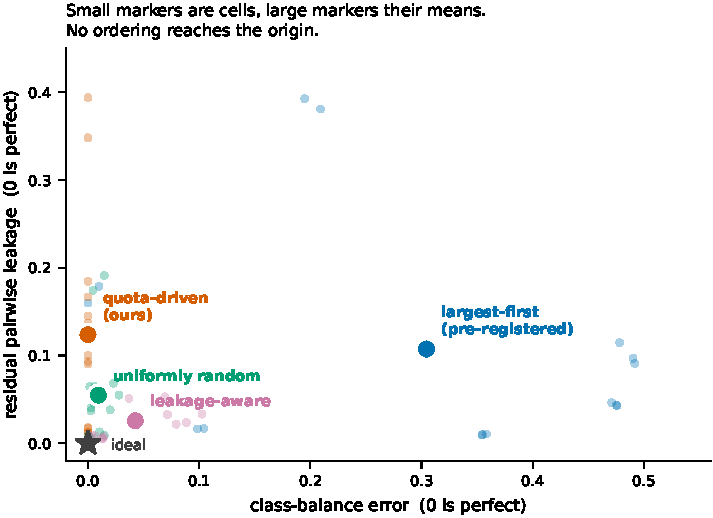
\includegraphics[width=0.66\textwidth]{F11_splitter_tradeoff.pdf}
\caption{Four cluster-disjoint orderings over identical clusterings. The ideal splitter
would sit at the origin and none does, which is the trade-off the text claims. The
informative part is where each lands: ordering by size costs class balance
(largest-first, far right), our quota-driven order buys exact balance at the highest
leakage of the four, and simply shuffling cluster order lands close to the origin on both.}
\label{fig:stress}
\end{figure}

\textbf{Uniformly random cluster order is the better default} (Figure~\ref{fig:stress}).
It reduces mean leakage by
more than half relative to our splitter ($0.055$ against $0.124$) and its worst case by a
factor of two ($0.191$ against $0.394$), at a balance error of $0.009$ -- not the exact
$0.000$ the quota-driven order achieves, but far below the $0.305$ of largest-first and well
inside what any downstream metric would notice. Leakage-aware ordering halves leakage again
($0.026$ mean, $0.053$ worst) at a balance error of $0.043$.

We therefore \textbf{withdraw the implicit recommendation} that a balance-preserving
splitter is the fix, and replace it with the weaker and better-supported claim: the problem
is \emph{size-ordered} cluster assignment, and simply shuffling cluster order removes most
of both artefacts at once. Our quota-driven splitter remains the right instrument for the
sensitivity analysis in this paper, because exact balance is what isolates the
class-balance artefact from everything else, and it is used only for that. It is not the
splitter we would now advise a benchmark to adopt. No ordering achieved all three targets,
so a benchmark must still report which it optimised and what it paid.

\subsection{The analysis plan, and every deviation from it}
\label{sec:prereg}

Because this paper argues that evaluation practice is unreliable, it would be
self-refuting to analyse it flexibly. We therefore wrote the hypotheses, the decision
thresholds and the power analysis before acquiring data, revised them once after the
design simulation and before any benchmark was obtained, and report every departure
below. We state the status of that document precisely, because overclaiming here would
undermine the rest of the paper.

\paragraph{What the plan is, and is not.} It is a dated analysis plan, written and revised
before execution, released in full with the harness. It was \textbf{not} deposited with a
third-party registry and carries \textbf{no external timestamp}; the only evidence of its
ordering is file modification time (plan last revised 2026-10-05; first Arm~B results
2026-10-06; Arm~A 2026-10-08) and the released history of the harness. We therefore
describe outcomes as \emph{pre-specified} rather than appealing to the stronger guarantee
that a registered pre-registration provides, and a reader is entitled to discount them
accordingly. We state the thresholds anyway, because a declared threshold that is kept
when it produces an unwelcome answer is still worth more than no threshold: ours produced
a null, and we report the null.

\paragraph{Pre-specified decision rules.} H1: mean pairwise $\tau_b$ across evaluation
levels is $<0.8$, confirmatory if the upper 95\% bound is below $0.8$. Co-primary:
normalised agreement $<0.85$ supports H1. Binding power statement: the design has 80\%
power only for a true mean $\tau_b \leq 0.646$, so an observation in $[0.65, 0.80]$ is
reported as inconclusive and not as a near-miss. Top-1 flip rate is descriptive and carries
no confirmatory weight. Secondary: H3, the negative-set variance component exceeds the
clustering-threshold component; H4, the seed component is under 25\% of the largest
protocol component; H5, representation ranks are less stable than learner ranks.

\paragraph{Deviations, in full.}
\begin{enumerate}[leftmargin=1.6em,itemsep=2pt]
\item \textbf{The unit of comparison in H1 changed, and this is the consequential
  deviation.} The plan expressed H1 over \emph{five independently published AMP
  benchmarks}. That comparison was not executed: the published resources do not share a
  task definition, a label convention or a redistributable positive set, and the
  pre-specified gate requiring us to reproduce each benchmark's own reported baseline to
  within $\pm 0.03$ could not be applied to resources whose headline numbers are not
  computed on a common target. We replaced it with the two crossed designs described
  above, in which the compared levels are five negative-set rules (Arm~B) and ten
  biological tasks (Arm~A). The estimator, the thresholds and the power statement were
  carried over unchanged, but \textbf{the hypothesis is tested over a different population
  of evaluation levels than the one originally named}, and the cross-benchmark question in
  its original form remains open. We flag this as the main reason to treat H1's status as
  pre-specified rather than pre-registered.
\item \textbf{Zoo size 12 $\to$ 20 pipelines} (and 16/24 as executed), after the design
  simulation improved minimum detectable disagreement from $\tau_b = 0.575$ to $0.646$.
  Made before any benchmark was acquired.
\item \textbf{Normalised agreement added as co-primary}, with the $0.85$ threshold, once
  the simulation showed $\tau_b$ cannot reach $1.0$ between seeds of one protocol.
\item \textbf{The RBF SVM became an approximation} (Nystr\"om, 512 components) on a
  measured 9-minute-per-cell exact fit. Validated after the fact in
  Section~\ref{sec:svm-validation}; the plan had listed this as available on request, and
  we have since done it.
\item \textbf{Thread caps and \texttt{tree\_method="hist"}} for XGBoost, on a measured
  $97\times$ scheduling artefact. Scheduling only; no model changed.
\item \textbf{End-to-end CNN/BiLSTM and ProtT5-XL excluded} as CPU-infeasible.
\item \textbf{The balance-preserving splitter and the entire second grid are post hoc},
  built after the pre-specified analysis returned a null. Reported as such throughout, and
  never as confirmatory (Section~\ref{sec:artefacts}).
\item \textbf{Residual-leakage measurement was added during execution}, replacing an
  assertion that failed on real data. It is a measurement we did not anticipate needing,
  not a changed outcome.
\end{enumerate}

Deviations 2--3 precede data acquisition; 4--6 were forced by timing measurements taken on
a single cell with no metric compared across pipelines; 1, 7 and 8 occurred during or after
execution and are the ones a reader should weigh.

\subsection{The four headline statistics, defined once}
\label{sec:definitions}

Four rank-agreement statistics appear in this paper and they compare different things. To
remove any ambiguity about which number refers to what, Table~\ref{tab:definitions} defines
each one, names the levels it compares, states how its ceiling is computed, and marks the
single \textbf{primary} result. Every later mention uses the labels in column~1, and no
other agreement numbers are quoted anywhere in the paper.

\begin{table}[htbp]\centering\small
\caption{The four rank-agreement statistics. All use mean pairwise \taub\ on MCC, over
pipelines ranked within a cell with ties averaged. The \emph{ceiling} is always the mean
\taub\ between \emph{seed pairs} holding every other factor fixed, so it measures
run-to-run reproducibility of the ranking under an unchanged protocol; \emph{normalised
agreement} is the ratio of the statistic to its own ceiling. \textbf{B1 is the primary
result}; B2 is a post hoc sensitivity analysis (Section~\ref{sec:artefacts}); B3 and A1 are
secondary. The pre-specified threshold is normalised agreement $<0.85$.}
\label{tab:definitions}
\begin{tabular}{llllcccl}
\toprule
Label & Levels compared & $n$ & Splitter & $\tau_b$ & ceiling & norm. & Status \\
\midrule
\textbf{B1} & negative-set rules & 5 & largest-first (pre-reg.) & 0.727 & 0.825 & \textbf{0.881} & \textbf{primary} \\
B2 & negative-set rules & 5 & balance-preserving & 0.693 & 0.867 & 0.800 & post hoc \\
B3 & clustering thresholds & 4 & largest-first (pre-reg.) & 0.817 & 0.825 & 0.990 & secondary \\
A1 & biological tasks & 10 & native (as released) & 0.479 & 0.838 & 0.572 & secondary \\
\bottomrule
\end{tabular}

\vspace{3pt}
\footnotesize\raggedright
Ceilings differ between B1/B3 and B2 because the ceiling is recomputed under whichever
splitter generated the partitions; it is a property of the protocol, not a constant. B1 and
B3 share a ceiling because they share the grid and differ only in which factor is varied.
\end{table}

\paragraph{Reading the primary result.} B1 is the pre-registered test and it is a
\textbf{null}: normalised agreement $0.881$ exceeds the $0.85$ threshold, so H1 is not
supported. B2 is the same comparison after a class-balance defect was corrected
(Section~\ref{sec:artefacts}); it falls below the threshold, but it was built after seeing
the null and is reported as a sensitivity analysis only. Any statement in this paper that
rankings disagree across protocols rests on B1, and B1 does not support it.

\subsection{Statistical analysis}

Pipelines are ranked within each cell with ties averaged, so we use \taub, which carries
the tie correction $\tau_a$ lacks. For each pair of levels we report the full matrix, its
mean, and the \textbf{top-1 flip rate}: the fraction of level pairs naming a different best
pipeline. Since leaderboards are read from the top, the latter is the quantity a
practitioner experiences.

\paragraph{The agreement ceiling.} $\tau_b$ does not reach $1.0$ even between two seeds of
the same protocol, because run-to-run noise reorders near-tied pipelines. We measure that
ceiling directly -- $\tau_b$ between seed pairs within a cell -- and report
\emph{normalised agreement}, the ratio of between-level $\tau_b$ to that ceiling. Reporting
raw $\tau_b$ alone invites comparison against $1.0$, which overstates disagreement. The
same reasoning is applied to the top-1 flip rate in Section~\ref{sec:flip-ceiling}, where
the ceiling turns out to matter more.

\paragraph{Variance decomposition on two responses.} The Arm~B grid is a complete balanced
factorial with one observation per cell, so method-of-moments variance components are exact
in closed form: the expected-mean-square equations solve top-down from the highest-order
interaction, which absorbs the residual. We report those as primary and sum-of-squares
shares ($\eta^2$) alongside them, since the two weight a factor's level count differently
and agreement between them is evidence that neither choice drives the conclusion.

We decompose both the metric score and the pipeline \emph{rank} within its cell, because a
factor can shift every score without changing any ranking, which is harmless to a
leaderboard, or reorder the top while barely moving scores, which is not. One caveat is
essential and we state it where the numbers appear
(Section~\ref{sec:structural-zero}): because ranks are assigned \emph{within} a cell, every
factor that helps define the cell has zero between-group variance on the rank response as
an algebraic identity, for any data whatsoever. The rank decomposition is therefore
informative about the pipeline main effect and the pipeline-by-factor interactions, and
says nothing at all about protocol main effects. Our claims about ordering rest on the
rank-agreement and flip-rate analyses instead.

\paragraph{Uncertainty, and the population each interval describes.} This deserves to be
stated explicitly, because our conclusions and our default intervals generalise over
different things.

Resampling \textbf{pipelines} answers: \emph{if we had drawn a different set of model
pipelines, how much would this agreement statistic move?} It holds the five rules or ten
tasks \textbf{fixed}, so it is an interval for these particular levels. That is the right
population for a claim about the zoo, and the wrong one for a claim about protocols or
tasks in general. All intervals labelled ``resampling pipelines'' are of this kind, and
they are our defaults because the pipeline is the unit the statistic is computed over.

Resampling \textbf{levels} answers the question our headline claims actually pose:
\emph{would another set of negative-set rules, or another set of tasks, give the same
answer?} We estimate it with a delete-one-level jackknife, the natural estimator here for
two reasons. First, the level is the sampling unit, so deleting one and recomputing
propagates exactly the dependence we care about. Second, a bootstrap that resamples levels
\emph{with replacement} is badly biased for this statistic: a duplicated level contributes a
pair with $\tau_b = 1$ by construction, which inflates agreement upward. Section~\ref{sec:level-uncertainty}
reports these intervals, and they are much wider than the pipeline intervals -- with five
rules and ten tasks they have to be. We therefore do not make population-wide claims about
protocols or tasks, and we say so in the abstract and the conclusion.

\paragraph{Dependence among level pairs.} Mean pairwise $\tau_b$ over $L$ levels averages
$L(L-1)/2$ pairs that are \textbf{not independent}: every level appears in $L-1$ of them, so
one unusual level perturbs many pairs at once. Treating pairs as independent units
understates uncertainty. The pair-level bootstrap in Table~\ref{tab:flipceiling} does
exactly that and is therefore anticonservative; we report it because it is the interval a
reader would otherwise compute, and we give the level jackknife beside it as the honest
alternative. The level jackknife is immune to this because it resamples levels, not pairs.

Variance-component intervals use a delete-one-seed jackknife, which preserves the balance
the decomposition requires. The two arms are compared by a paired bootstrap over the shared
pipelines \emph{and}, in Section~\ref{sec:level-uncertainty}, by a two-sample level
jackknife; a permutation test swapping rows between arms is unavailable because the arms
have ten and five levels respectively.

\subsection{Computational notes}

Three measured costs shaped the executed configuration, each reported because it is easy to
get wrong in the same way we initially did. Sorting sequences by length before batching
reduced ESM-2 8M embedding from 959 to \SI{2.1}{\milli\second} per sequence and 650M from
2008 to \SI{91.6}{\milli\second}, because unsorted batches pad every member to the longest.
Capping worker threads at 8 reduced a gradient-boosting fit on a seven-feature problem from
\SI{165}{\second} to \SI{1.7}{\second}, nested parallelism having oversubscribed a
32-thread machine. An exact RBF SVM with probability calibration did not complete one cell
in nine minutes, motivating the Nystr\"om approximation. None was chosen after seeing a
ranking.

\subsection{Validating the kernel approximation}
\label{sec:svm-validation}

The Nystr\"om substitution is the only change we make to a model rather than to its
scheduling, so we validated it directly. We re-ran the physicochemical/SVM pipeline with an
exact RBF kernel and probability calibration across all five negative rules at three seeds
(15 matched cells), holding the split, the feature matrix and the hyperparameters fixed, and
capping the training set at 2000 sequences so the exact fit was tractable.

Scores track closely. Mean AUROC was 0.799 exact against 0.770 approximate (mean absolute
difference 0.044, maximum 0.114); mean MCC was 0.336 against 0.311 (mean absolute difference
0.031, maximum 0.071). Across the 15 cells the two variants correlate at $r = 0.997$ on MCC
and $r = 0.969$ on AUROC, with Kendall $\tau_b = 0.810$ and $0.829$ respectively. The
rule-level ordering, which is the quantity this paper measures, is preserved exactly on
AUROC ($\tau_b = 1.000$) and to one adjacent inversion on MCC ($\tau_b = 0.800$). The
approximation was 105-fold cheaper (\SI{0.6}{\second} against \SI{61.6}{\second} per fit),
which is what made the full grid feasible. Per-cell values are in
\texttt{tables/svm\_approximation\_check.csv}.

The approximation is therefore slightly pessimistic in absolute score -- it costs about
0.03--0.04 of both metrics -- but does not reorder the protocol comparison. We treat it as
a validated substitution rather than an open caveat.

%=======================================================================
\section{Arm B: varying the evaluation protocol}
%=======================================================================

\subsection{The five negative-set rules pose measurably different problems}

Positives: 5{,}187 peptides, median length 18, mean net charge $+4.21$.
Table~\ref{tab:ladder} shows that the rules form an ordered ladder of which shortcuts
survive.

\begin{table}[htbp]\centering\small
\caption{Corpus characterisation. Matching negative length removes the length artefact
exactly but \emph{quadruples} the net-charge gap, because length-matched fragments come
from near-neutral protein interiors while antimicrobial peptides are strongly cationic.}
\label{tab:ladder}
\begin{tabular}{lrrrr}
\toprule
Negative-set rule & Neg.\ median length & Length ratio & Charge gap & Comp.\ $L_1$ \\
\midrule
random UniProt       & 73 & 4.06 & 1.01 & 1.206 \\
annotation filtered  & 75 & 4.17 & 0.99 & 1.201 \\
length matched       & 18 & 1.00 & \textbf{4.25} & 1.270 \\
composition matched  & 18 & 1.00 & 2.57 & 0.796 \\
shuffled positives   & 18 & 1.00 & \textbf{0.00} & \textbf{0.000} \\
\bottomrule
\end{tabular}
\end{table}

\begin{figure}[htbp]\centering
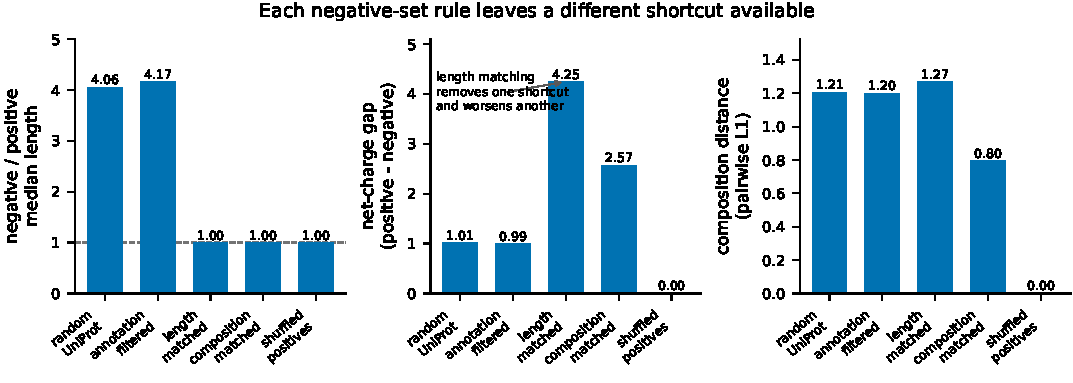
\includegraphics[width=\textwidth]{F1_shortcut_ladder.pdf}
\caption{Each negative-set rule leaves a different shortcut available. The middle panel is
the counterintuitive one: the standard remedy for the length artefact makes the charge
artefact four times stronger.}
\label{fig:ladder}
\end{figure}

\subsection{Protocol choice transforms apparent difficulty}

Mean MCC over the pipelines spans \textbf{0.311 to 0.913} across the twenty protocol cells
(Figure~\ref{fig:landscape}). The same pipelines on the same positive set produce results
from barely-better-than-chance to near-perfect, depending on choices a methods section
usually compresses into one sentence.

\begin{figure}[htbp]\centering
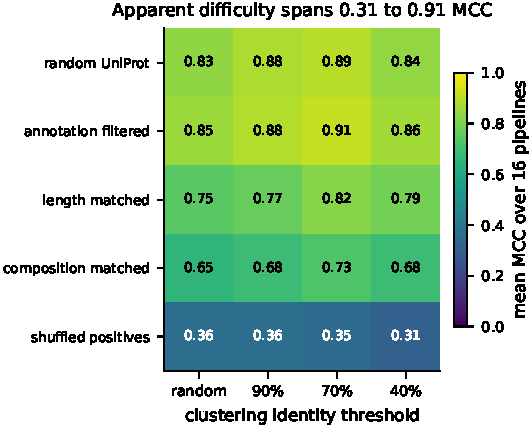
\includegraphics[width=0.62\textwidth]{F2_performance_landscape.pdf}
\caption{Mean MCC by negative-set rule and clustering threshold.}
\label{fig:landscape}
\end{figure}

\subsection{The ordering is largely preserved; the winner is not}
\label{sec:tau-protocol}

\textbf{Two different questions, kept apart.} ``Do protocols agree?'' has two answers that
point in opposite directions, and conflating them is how this literature reaches
overconfident conclusions in either direction. We therefore report them separately
throughout:

\begin{itemize}[leftmargin=1.4em,itemsep=1pt]
\item \textbf{Broad ordering} -- does the whole leaderboard keep its shape? Measured by mean
  pairwise $\tau_b$ against its seed ceiling. Answer: \emph{largely, but not entirely}.
\item \textbf{Winner identity} -- does the same pipeline come first? Measured by the top-1
  flip rate against its own seed ceiling (Section~\ref{sec:flip-ceiling}). Answer:
  \emph{often not}.
\end{itemize}

On the primary analysis \textbf{B1}, mean pairwise $\tau_b$ across the five rules is
$0.727$ against a measured seed ceiling of $0.825$: normalised agreement $\mathbf{0.881}$,
\emph{above} the pre-specified threshold of $0.85$, so H1 is \textbf{not supported}. Under
the post hoc \textbf{B2} the same comparison gives $\tau_b = 0.693$ against a ceiling of
$0.867$, normalised $0.800$ (Section~\ref{sec:artefacts}; labels as in
Table~\ref{tab:definitions}).

The broad ordering is therefore stable but \emph{not} fixed, and we want to be careful not
to overstate the stability either. A normalised agreement of $0.881$ means roughly
one-eighth of the reproducible ordering is lost to protocol choice, and the largest rank
swing is 7 of 16 positions (Figure~\ref{fig:bump}) -- rankings do change. What does not
happen is wholesale scrambling: the weakest pipelines stay at the bottom under every rule.

Winner identity behaves differently. \textbf{9 of 10 rule pairs name a different best
pipeline}, with four distinct winners. This is not in conflict with the high $\tau_b$:
$\tau_b$ weights all 120 pairwise orderings equally and most are stable, while the leading
places -- which are close in score -- reorder. Section~\ref{sec:flip-ceiling} shows how much
of that reordering exceeds run-to-run noise, and Section~\ref{sec:level-uncertainty} how
precisely five rules can locate it.

\begin{figure}[htbp]\centering
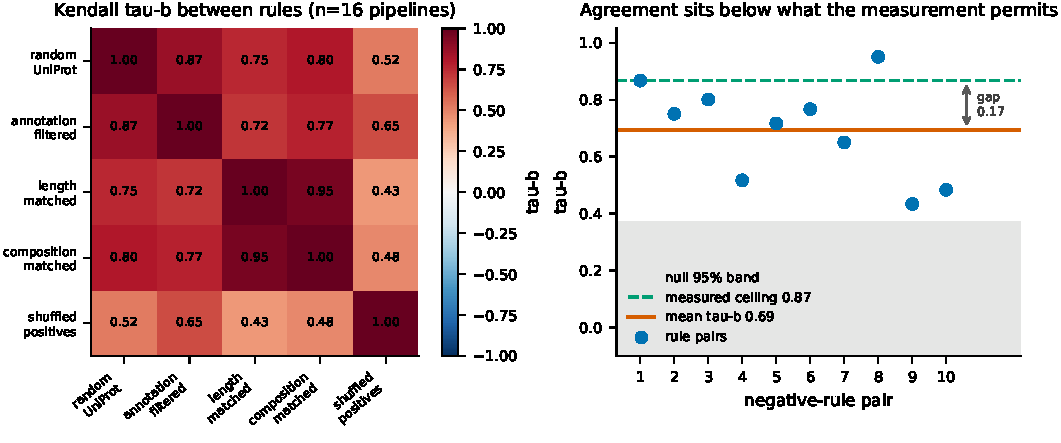
\includegraphics[width=\textwidth]{F4_agreement_vs_ceiling.pdf}
\caption{Left: $\tau_b$ between every pair of negative-set rules. Right: the ten pair
values against the \emph{measured} seed ceiling and against the permutation null band.
Agreement sits well above chance and clearly below what the measurement permits -- the gap
the normalised statistic quantifies. This, not the rank-variance decomposition, is the
direct evidence for the ordering claim.}
\label{fig:agreement}
\end{figure}

\begin{figure}[htbp]\centering
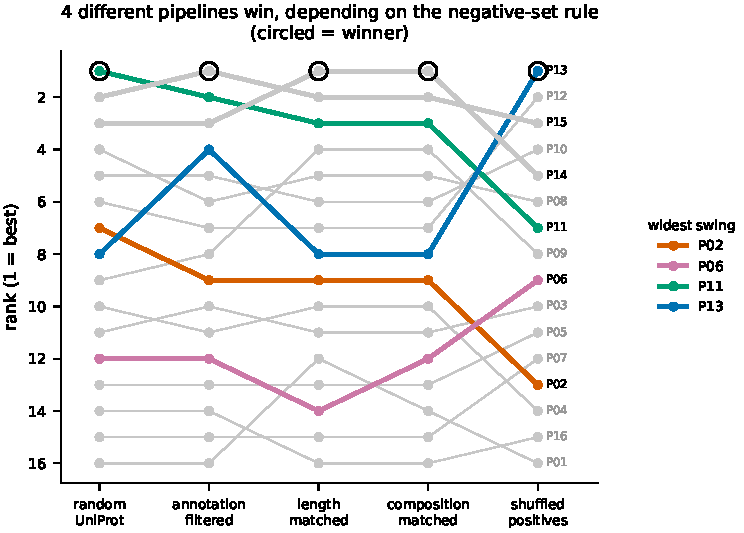
\includegraphics[width=0.8\textwidth]{F3_bump_chart.pdf}
\caption{Pipeline rank against negative-set rule. Circled markers are the winner under each
rule.}
\label{fig:bump}
\end{figure}

Clustering threshold leaves the \emph{ordering} untouched. Under the pre-registered
splitter $\tau_b = 0.817$ against a ceiling of $0.825$, a normalised agreement of $0.990$;
under the balance-preserving splitter $\tau_b = 0.889$ against $0.867$, i.e.\ normalised
$1.03$ -- at or above the ceiling, meaning the threshold reorders pipelines no more than
reseeding the same protocol does.

Its effect on the \emph{winner} depends on how much averaging is done first, and we were
initially too quick here. Scoring each pipeline on its mean over all five seeds and all
five rules, no threshold pair changes the winner ($0$ of $6$). But a published benchmark
reports one run, not a mean over twenty, and at single-run resolution -- holding the rule
and seed fixed and comparing thresholds -- the winner changes in $75.3\%$ of pairs, against
a seed-noise ceiling of $54.5\%$ (difference ${+}0.208$, $[{+}0.110, {+}0.305]$ over pairs;
Section~\ref{sec:flip-ceiling}). That is close to the negative rule's $76.0\%$. Both
figures are descriptive of these four thresholds and five rules: the interval resamples
pairs drawn from a handful of levels, and resampling the levels instead leaves the
threshold flip rate wholly undetermined, $[0.000, 1.000]$
(Section~\ref{sec:level-uncertainty}).

We therefore make the narrower claim the data support: \textbf{within this corpus the
threshold is benign for the ordering but not for the winner}, and the negative-set rule is
the factor that damages both. Read as an observation about current practice rather than as
an inference, the field has standardised the factor that is harmless to the ranking and
left unstandardised the factor that is not.

\subsection{What moves the score is not what moves the ranking}

\subsubsection*{Score: the negative-set rule owns most of the variance}

Table~\ref{tab:variance} decomposes the MCC of the complete balanced factorial
(16 pipelines $\times$ 5 rules $\times$ 4 thresholds $\times$ 5 seeds, one observation per
cell) two ways. The negative-set rule is the largest single component on either measure:
$\hat\sigma^2 = 0.0467$, \textbf{71.0\%} of the total estimated variance, against
$14.8\%$ for the pipeline itself. \textbf{Which negatives a benchmark invents matters more
to the number it reports than which model is run on it.} The clustering threshold accounts
for $0.6\%$ and the seed for a component estimated at $-1\times10^{-6}$,
i.e.\ indistinguishable from zero.

The two columns are different estimators of the same thing and agree closely, which is why
we show both. Moment-based variance components put each factor on a common footing
regardless of how many levels it has; sums-of-squares shares ($\eta^2$) do not, and favour
factors with more levels. Agreement to within four percentage points means the conclusion
is not an artefact of either choice. We report the moment estimates as primary: the design
is a complete balanced factorial, so the expected-mean-square equations solve exactly in
closed form, whereas a REML fit of the same crossed model lands on the parameter boundary
and does not converge.

\begin{table}[htbp]\centering\small
\caption{Variance decomposition of MCC in Arm~B. Columns 2--3 are exact method-of-moments
variance components; column 4 is the sum-of-squares share of the same model, shown to
demonstrate the two estimators agree. Column 5 is the sum-of-squares share on the
\emph{rank} response, with delete-one-seed jackknife intervals. Protocol main effects are
\emph{structurally} zero on rank -- see the text; this is an identity, not a measurement.}
\label{tab:variance}
\begin{tabular}{lrrrcr}
\toprule
 & \multicolumn{3}{c}{score (MCC)} & \multicolumn{2}{c}{rank} \\
\cmidrule(lr){2-4}\cmidrule(lr){5-6}
Component & $\hat\sigma^2$ & \% $\hat\sigma^2$ & \% SS & \% SS & 95\% CI \\
\midrule
negative rule               & 0.0467 & \textbf{71.0} & 67.9 & $0$\textsuperscript{$\dagger$} & -- \\
clustering threshold        & 0.0004 &  0.6 &  0.7 & $0$\textsuperscript{$\dagger$} & -- \\
threshold $\times$ rule     & 0.0003 &  0.5 &  0.4 & $0$\textsuperscript{$\dagger$} & -- \\
seed                        & $<10^{-5}$ &  0.0 &  0.0 & $0$\textsuperscript{$\dagger$} & -- \\
\addlinespace
pipeline                    & 0.0098 & 14.8 & 19.2 & 83.47 & $[82.83,\ 84.11]$ \\
pipeline $\times$ rule      & 0.0073 & \textbf{11.0} & 10.0 & \textbf{8.87} & $[8.30,\ 9.43]$ \\
pipeline $\times$ threshold & 0.0005 &  0.8 &  0.8 & 1.26 & $[0.97,\ 1.55]$ \\
\bottomrule
\end{tabular}

\vspace{2pt}
\footnotesize\raggedright
\textsuperscript{$\dagger$}Identically zero for any dataset, because ranks are assigned
within a cell: see Section~\ref{sec:structural-zero}.
\end{table}

\begin{figure}[htbp]\centering
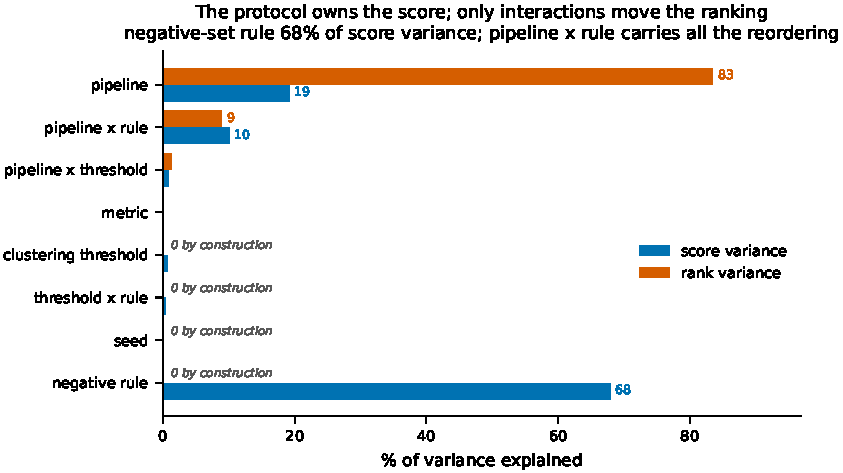
\includegraphics[width=0.78\textwidth]{F5_variance_decomposition.pdf}
\caption{Score variance against rank variance by component.}
\label{fig:variance}
\end{figure}

\subsubsection*{Rank: why the protocol main effects are zero by construction}
\label{sec:structural-zero}

Repeating the decomposition on the within-cell rank returns \emph{exactly} zero for every
protocol main effect. We initially read this as a striking empirical result. It is not: it
is an algebraic identity, and we state it as one because the arithmetic is worth having in
the open.

Ranks are assigned to the $K$ pipelines separately within each
(metric, threshold, rule, seed) cell. Every cell therefore contains each rank exactly once,
so the mean rank in every cell is $(K+1)/2$ regardless of the scores. Any factor that helps
\emph{define} the cell partitions the data into groups of whole cells, so each of its group
means is also $(K+1)/2$, and its between-group sum of squares is identically zero. We
verified this numerically -- the mean rank is $8.500$ for all five rules, all four
thresholds and all five seeds, with $K=16$ -- but no verification was needed. The
jackknife interval $[0.00, 0.00]$ and standard error of $0.00$ we previously reported are
the signature of a constant, not evidence of a precisely measured null.

This is not a defect of the rank response; it is the reason rank-based analysis is the
right instrument. A factor that shifts every score in a cell by the same amount cannot
touch the ordering, and the decomposition records that by construction. But it means the
rank column cannot be used to argue that protocol choice \emph{happens} not to reorder
pipelines, and we no longer do so. On the rank response the informative terms are the
pipeline main effect and the pipeline-by-factor interactions, which are free to vary and do:

\begin{itemize}[leftmargin=1.4em,itemsep=1pt]
\item pipeline $\times$ rule accounts for $8.87\%$ $[8.30, 9.43]$ of rank variance,
  \textbf{seven times} the pipeline $\times$ threshold term ($1.26\%$ $[0.97, 1.55]$).
  All reordering attributable to the protocol is carried by these interactions, and the
  negative-set rule dominates the threshold within them.
\item On the score response the same two terms are $11.0\%$ and $0.8\%$ --
  the only components whose relative standing is similar across the two responses, because
  an interaction is precisely a term that moves pipelines differentially.
\end{itemize}

The substantive claim of this section therefore rests on the direct rank-agreement
evidence of Sections~\ref{sec:tau-protocol} and~\ref{sec:flip-ceiling}, not on the
zero entries in Table~\ref{tab:variance}. What the decomposition does establish is the
\emph{score} result: a single protocol choice owns $71\%$ of the variance in reported
performance, seven times the pipeline's own $14.8\%$.

\subsection{The null baseline tracks the shortcut ladder}

A two-feature pipeline (length, net charge) reaches MCC $0.793$ on proteome-derived
negatives, within $0.11$ of a 650M-parameter language model, and falls to
$\mathbf{-0.074}$ -- below chance -- on shuffled positives, where length, charge and
composition are identically zero by construction (Figure~\ref{fig:null}). The progression
was predicted from Table~\ref{tab:ladder} before the grid was run.

\begin{figure}[htbp]\centering
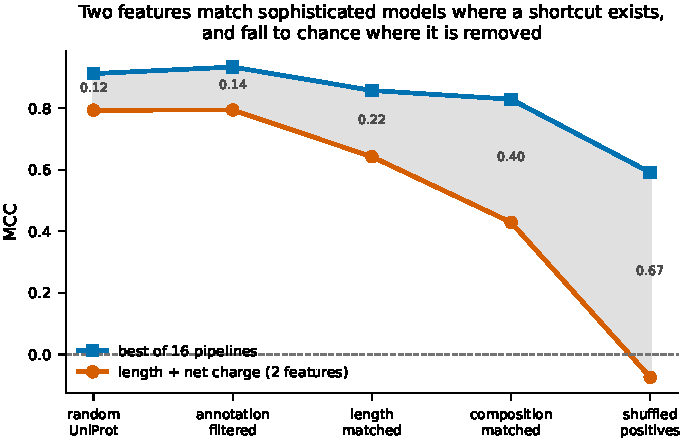
\includegraphics[width=0.62\textwidth]{F6_null_baseline.pdf}
\caption{The two-feature baseline against the best of the zoo, by negative-set rule.}
\label{fig:null}
\end{figure}

\textbf{A benchmark whose negatives are drawn as whole proteome sequences is substantially
solvable without any model of antimicrobial activity.}

\subsection{Class provenance is asymmetric under two of the five rules}
\label{sec:exposure}

Two of our five negative-set rules draw their negatives \emph{from} reviewed UniProt, while
the positives come from DBAASP. The two classes therefore differ in provenance, not only in
activity, and that raises a question for any model pretrained on proteomes: is one class
made of ordinary proteome entries and the other not?

Table~\ref{tab:exposure} measures it. Under those two rules the asymmetry is close to
total: \textbf{100\% of negatives and $7.9\%$ of positives} are verbatim entries in the
reviewed UniProt release we retrieved, a 92-point gap aligned with the class label. Under
the three rules that synthesise negatives from the positives -- length matched, composition
matched, shuffled -- negative overlap falls to $0.06\%$ or below and the gap nearly
vanishes.

\paragraph{This is an overlap audit against current UniProt, not a measurement of ESM-2's
training data.} We are explicit about that because the tempting stronger claim is not
supported, and an earlier draft of this section made it. ESM-2 was pretrained on UniRef
derived from UniProt release \textbf{2021\_04}~\citep{lin2023esm2}; our audit uses reviewed
UniProt retrieved \textbf{2026-10-05}. Overlap with the latter neither implies nor excludes
presence in the former, and it fails in \emph{both} directions:

\begin{itemize}[leftmargin=1.4em,itemsep=1pt]
\item a sequence in the 2026 release may have been deposited after 2021\_04 and so was never
  available to the model, so overlap is not a lower bound on exposure;
\item UniRef is built from the whole of UniProt, whereas we checked only the \emph{reviewed}
  subset -- about $4.9\times10^{5}$ sequences against the order of $10^{8}$ in UniProt
  overall -- so a sequence absent from our audit may still have been in training, and
  non-overlap is not an upper bound either.
\end{itemize}

Establishing exposure would mean reconstructing the 2021\_04 UniRef50/90 release and
checking membership there, cluster-representative status included. We have not done that.
What the audit does establish is a fact about the benchmark rather than about the model:
\textbf{under the two proteome-derived rules one class consists entirely of ordinary
reviewed-proteome entries and the other almost entirely does not.} Any encoder pretrained
on proteomes is then asked to separate two classes that differ in provenance as well as in
antimicrobial activity -- a route to a high score that is not a model of the property, and
one available independently of the length and charge shortcuts.

\begin{table}[htbp]\centering\small
\caption{Exact sequence membership in reviewed UniProt as retrieved 2026-10-05, by
negative-set rule and class. This is an overlap audit against the current release, not a
reconstruction of any model's training set. The positive set is identical across rules by
construction, so its $7.9\%$ is a constant; what varies is the negatives.}
\label{tab:exposure}
\begin{tabular}{lrrrr}
\toprule
 & \multicolumn{2}{c}{negatives in UniProt} & \multicolumn{2}{c}{positives in UniProt} \\
\cmidrule(lr){2-3}\cmidrule(lr){4-5}
Negative-set rule & $n$ & \% & $n$ & \% \\
\midrule
random UniProt       & 5{,}187 & \textbf{100.00} & 410 & 7.9 \\
annotation filtered  & 5{,}187 & \textbf{100.00} & 410 & 7.9 \\
composition matched  &       3 & 0.06            & 410 & 7.9 \\
length matched       &       1 & 0.02            & 410 & 7.9 \\
shuffled positives   &       0 & 0.00            & 410 & 7.9 \\
\bottomrule
\end{tabular}
\end{table}

\begin{figure}[htbp]\centering
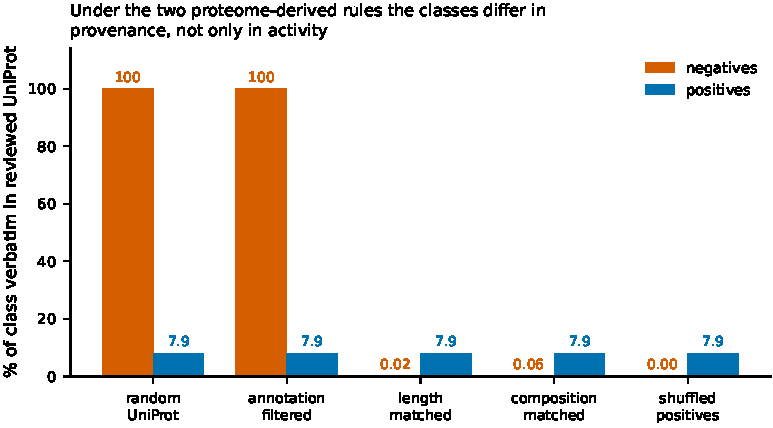
\includegraphics[width=0.68\textwidth]{F13_provenance.pdf}
\caption{Percentage of each class that is a verbatim entry in reviewed UniProt as retrieved
2026-10-05. The positive set is fixed across rules, so its $7.9\%$ is a constant and only
the negatives move. Under the two proteome-derived rules the classes differ almost
completely in provenance; under the three synthesised rules they do not. This is an overlap
audit against the current release, not a measurement of any model's training set.}
\label{fig:provenance}
\end{figure}

\textbf{A provenance shortcut, independent of length and charge.} The two rules whose
negatives are wholly proteome-derived are the same two on which the two-feature baseline
reaches MCC $0.79$ and mean MCC reaches $0.91$. A benchmark built that way offers two
unrelated routes to a high score -- the compositional shortcut of the ladder above, and
discriminating proteome entries from synthetic peptides on whatever regularities distinguish
them -- and neither is a model of antimicrobial activity. We cannot separate the two routes
with this design, and we make no claim about what the ESM-2 pipelines actually use; the
point is that the benchmark cannot distinguish them either.

\paragraph{The same audit on Arm~A.} Of 9{,}655 distinct test sequences across the ten
tasks, $12.1\%$ are verbatim reviewed-UniProt entries, and the rate varies enormously by
task: \textbf{toxicity $55.8\%$}, antifungal $26.3\%$, antimicrobial $11.9\%$, neuropeptide
$11.7\%$, down to DPP-IV $1.2\%$ and ACE-inhibitory $1.9\%$
(\texttt{tables/esm\_exposure\_audit.csv}). Toxicity is also the task where cluster-disjoint
splitting inverts the sign of net charge (Section~\ref{sec:artefacts}c), so it is at once the
most proteome-like and the most shifted of the ten. Because provenance varies across tasks by
a factor of 45 it is a plausible contributor to the poor rank transfer of Arm~A, and it is
not something any leaderboard currently reports. The same caveat applies as above: this
describes what the datasets are made of, not what any model was trained on.

\subsection{Would an equal tuning budget change the answer?}
\label{sec:tuning}

Fixing hyperparameters across every cell is what keeps protocol preference from
being confounded with search effort, but it leaves a fair objection standing: a fixed
setting may suit a random forest better than an MLP, so part of the ranking could reflect
whose defaults were luckier rather than whose method is better.

We tested it by giving every pipeline the \textbf{same budget} -- six candidate
configurations for each of the five learners -- and selecting among them on a validation
split taken from inside the training partition. Two properties are enforced: the inner
split is \textbf{cluster-disjoint}, using the clustering that produced the outer split, so
hyperparameters are not chosen on sequences homologous to those they are validated against;
and the \textbf{test partition is untouched} during selection, scored once after refitting
the chosen configuration on the full training partition. Five rules at threshold $0.7$,
seed $0$, the 16 Arm~B pipelines: 560 fits.

\begin{table}[htbp]\centering\small
\caption{Equal tuning budget against the fixed hyperparameters used throughout. Agreement
across rules is the quantity the paper's conclusions rest on, and tuning does not move it.
The within-rule comparison is given against the seed ceiling for the same design, which is
the right scale for judging it.}
\label{tab:tuning}
\begin{tabular}{lcc}
\toprule
 & fixed & equal budget \\
\midrule
mean test MCC over 80 pipeline-rule cells & 0.487 & 0.491 \\
mean pairwise $\tau_b$ \emph{across rules} & 0.563 & 0.587 \\
\addlinespace
\multicolumn{3}{l}{\emph{within-rule, fixed ranking against tuned ranking}} \\
\quad mean $\tau_b$ & \multicolumn{2}{c}{0.843 \quad(min 0.783)} \\
\quad seed ceiling, same design & \multicolumn{2}{c}{0.867} \\
\quad rules whose winner changes & \multicolumn{2}{c}{3 of 5} \\
\bottomrule
\end{tabular}
\end{table}

\textbf{The conclusions do not change.} Agreement across the five rules is $0.563$ with
fixed hyperparameters and $0.587$ with an equal budget: tuning does not rescue
cross-protocol agreement, which is the claim that would have been in danger. The mean gain
from tuning is $+0.005$ MCC, with a maximum of $+0.056$ -- the fixed settings were close to
the best of six for most pipelines.

\textbf{There is a mild family bias, in the direction the objection anticipated.} Mean gain
by learner is $+0.017$ for the approximate SVM and $+0.010$ for gradient boosting, against
$+0.004$, $+0.003$ and $+0.002$ for logistic regression, random forest and the MLP. The
fixed defaults suited the kernel machine and the booster least. The effect is real and we
report it, but it is about $0.02$ MCC, against the $0.6$ MCC that separates the easiest
protocol cell from the hardest: a thirtieth of the effect the paper is about.

\textbf{Tuning does move the winner, and the reason is the paper's own thesis.} Three of
five rules crown a different pipeline under tuning, and the fixed-versus-tuned ranking
agreement, $\tau_b = 0.843$, is slightly below the seed ceiling of $0.867$ for the same
design -- so tuning perturbs the ranking about as much as reseeding does, marginally more.
Inspecting the three changes shows what they are: under annotation-filtered negatives the
winner moves from P14 at MCC $0.960$ to P10 at $0.958$, under composition-matched from P10
at $0.340$ to P13 at $0.342$, under length-matched from P08 at $0.430$ to P12 at $0.439$.
These are near-ties decided by the third decimal. They do not show that tuning changes
which method is better; they show again that the top of this leaderboard is a near-tie that
any perturbation reorders (Section~\ref{sec:flip-ceiling}).

\subsection{Metric choice reorders models about as much as the negative rule}

Mean pairwise $\tau_b$ between the six metrics, protocol averaged out, is $0.780$ --
comparable to the $0.693$ between negative rules. Accuracy against AUPRC is $0.617$.
Entered as an explicit factor, metric accounts for $31.1\%$ of score variance, exceeding
the negative-set rule.

\subsection{Is it the rule, or the particular negatives it happened to draw?}
\label{sec:draw}

The main grid embeds \textbf{one} negative realisation per rule, because embedding five
draws at four ESM-2 scales was not affordable on CPU. The reported seed component therefore
varies the partition and the model initialisation but not \emph{which} negatives were
sampled, and a rule effect estimated from a single draw could in principle be that draw's
idiosyncrasy rather than the rule's.

We close this on the twelve embedding-free pipelines, where no ESM cache is needed: five
independent negative pools per rule, 25 cells at the $0.7$ threshold, with the seed held
fixed so the draw is the only thing moving. The seed ceiling and the across-rule value are
recomputed on the \emph{same} twelve pipelines at the same threshold, so all three numbers
in Table~\ref{tab:draw} are comparable; they are not comparable to the 16-pipeline
statistics elsewhere in the paper, and we do not mix them.

\begin{table}[htbp]\centering\small
\caption{Three sources of ranking movement, measured on one matched design: 12
embedding-free pipelines, threshold $0.7$. \emph{Normalised} divides by the seed ceiling,
which is itself computed on these twelve pipelines. The negative-set rule disturbs the
ranking roughly twice as much as redrawing the negatives within a rule, which is the
reassurance the main grid needed; but the draw is not negligible, and for the two matched
rules it approaches the rule effect.}
\label{tab:draw}
\begin{tabular}{lcc}
\toprule
What varies & mean $\tau_b$ & normalised \\
\midrule
seed only: partition and initialisation (the ceiling) & 0.857 & 1.000 \\
\textbf{negative draw}, within a rule                 & 0.728 & 0.849 \\
\textbf{negative rule}                                & 0.357 & \textbf{0.417} \\
\midrule
\multicolumn{3}{l}{\emph{per-rule draw agreement}} \\
\quad shuffled positives   & 0.867 & 1.011 \\
\quad random UniProt       & 0.818 & 0.955 \\
\quad annotation filtered  & 0.806 & 0.940 \\
\quad length matched       & 0.590 & \textbf{0.688} \\
\quad composition matched  & 0.559 & \textbf{0.653} \\
\bottomrule
\end{tabular}
\end{table}

\begin{figure}[htbp]\centering
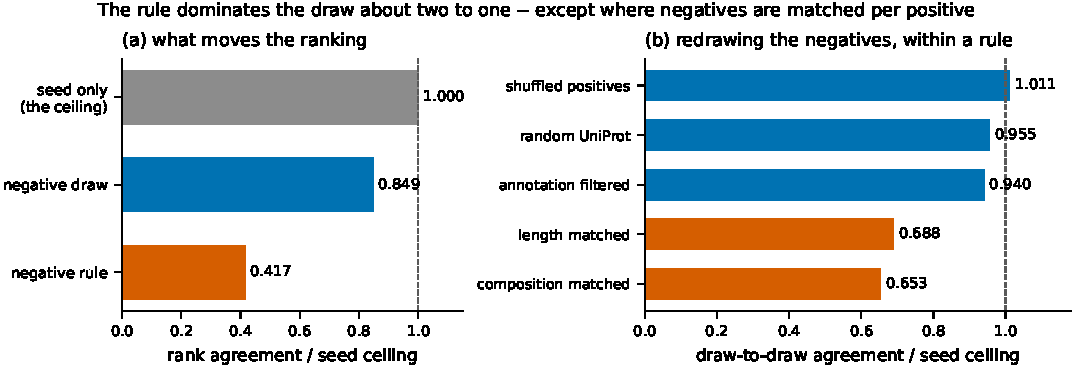
\includegraphics[width=\textwidth]{F10_draw_sensitivity.pdf}
\caption{(a) The negative-set rule disturbs the ranking about twice as much as redrawing
the negatives within a rule, both read against the seed ceiling. (b) That average hides the
important part: for the three rules whose negatives are either deterministic or drawn from
a very large pool, redrawing changes almost nothing, while for the two \emph{matched} rules
-- the ones designed to remove the length and composition shortcuts -- the draw alone moves
the ranking to $0.65$--$0.69$ of the ceiling.}
\label{fig:draw}
\end{figure}

\textbf{The main conclusion survives: the rule dominates the draw}, by roughly a factor of
two on the normalised scale ($0.417$ against $0.849$; Figure~\ref{fig:draw}a). Fixing the
realisation did not manufacture the disagreement we attribute to the negative-set rule.

\textbf{But the draw is a real source of variation, and it is concentrated in exactly the
rules the field would consider most careful.} For shuffled positives and the two
proteome-derived rules, redrawing the negatives leaves the ranking essentially at the
ceiling ($0.94$--$1.01$ normalised): those constructions are stable because they are either
deterministic given the positives or sampled from a pool so large that any two draws look
alike. For \textbf{length matched} and \textbf{composition matched} -- the rules designed to
remove the length and composition shortcuts, and therefore the ones a careful benchmark is
most likely to adopt -- normalised draw agreement falls to $0.688$ and $0.653$. Each
matched negative is chosen per-positive from a candidate pool, so two draws under the same
rule yield materially different problems.

Two consequences we would rather state than have inferred. First, for those two rules the
single-draw rule effect reported in the main grid is partly draw-specific, and the honest
reading of a matched-negative benchmark is that \emph{the rule does not determine the
benchmark} -- the realisation has to be published alongside it. Second, our seed component
understates total run-to-run variability for those rules, because the draw sits outside it;
the decomposition in Table~\ref{tab:variance} should be read as conditional on the
realisation rather than marginal over it. A benchmark reporting a matched-negative result
from one draw is reporting something less reproducible than its seed variance suggests.

%=======================================================================
\section{Arm A: varying the biological task}
%=======================================================================

\subsection{Rankings transfer poorly across tasks}

Holding the protocol fixed and varying the task gives mean pairwise $\tau_b = 0.479$
$[0.351, 0.564]$ against a measured ceiling of $0.838$, a normalised agreement of
$\mathbf{0.572}$. The null standard deviation of the mean statistic for this design is
$0.022$, so this is far from chance and equally far from transfer.

\textbf{42 of 45 task pairs name a different best pipeline} (flip rate $0.933$
$[0.800, 0.956]$), with \textbf{seven distinct winners} across ten tasks and a largest rank
swing of \textbf{20 of 24 positions}. A method selected on antimicrobial data carries
little information about which method will win on toxicity.

\subsection{Difficulty varies as much across tasks as across protocols}

Mean MCC over 24 pipelines ranges from $0.608$ (tumour T-cell antigen) to $0.254$
(anticancer), with antimicrobial at $0.255$ -- far below the $0.91$ the same pipelines
reach on proteome-derived negatives in Arm~B. The difference is not the methods; it is that
these benchmarks use curated negatives rather than arbitrary proteome sequences. This is
the clearest demonstration of the Arm~B finding: \textbf{the negative-set rule, not the
method, sets the achievable number.}

\subsection{The null baseline behaves oppositely here, and that is the point}

Across all ten tasks the two-feature baseline ranks 20th to 24th of 24, with margins to the
best pipeline from $0.17$ to $0.68$. On proteome-derived negatives in Arm~B the same two
features reached $0.79$. \textbf{The shortcut was never a property of peptide prediction;
it was a property of how the negatives were drawn.}

\subsection{Three further artefacts of homology-aware splitting}
\label{sec:artefacts}

\subsubsection*{(a) Cluster-disjoint is not pairwise-disjoint}

Greedy clustering does not form equivalence classes, so two sequences can occupy different
clusters and still exceed the identity threshold. Measured in-grid, the fraction of test
sequences with an above-threshold hit in training rises from $1.41\%$ at a 90\% threshold
to $\mathbf{21.63\%}$ at 40\%, reaching $39\%$ for whole-protein negatives across 45
independent splits. \textbf{The stricter the nominal threshold, the more leakage survives},
because a loose criterion admits far more qualifying pairs and short peptides clear 40\%
identity by chance. The effect is unchanged under the balance-preserving splitter
($22.99\%$ at 40\%), confirming it is a property of cluster-disjoint splitting itself.

\subsubsection*{(b) It destroys class balance}

On a corpus balanced 1:1 by construction, test-set positive fraction reaches
$\mathbf{99.5\%}$ at the 40\% threshold. The mechanism is rule-dependent: antimicrobial
peptides are homologous to one another and form large clusters, so largest-first assignment
sends them to the test partition, while negatives derived \emph{from} the positives remain
singletons. Whole-protein negatives form their own families and occupy the test partition
instead, inverting the imbalance to $0.29$.

Our balance-preserving splitter (Section~\ref{sec:balanced}) restores the test positive
fraction to $0.500$ in \textbf{all fifteen} rule-by-threshold configurations, holds the
test fraction at exactly $0.200$, and never splits a cluster. Re-running the full grid with
it \textbf{strengthens every finding}: normalised agreement falls $0.881 \to 0.800$, winner
flips rise $7/10 \to 9/10$, and the pipeline-by-rule rank-variance share rises
$6.9\% \to 8.9\%$ (Figure~\ref{fig:balanced}). The imbalance had been \emph{masking}
disagreement, because a 99\%-positive test set compresses MCC and makes pipelines bunch.

\paragraph{Status of this analysis.} The splitter was built after observing that the
pre-registered analysis did not support our hypothesis. Its motivation was a verification
failure logically independent of the ranking result, but the ordering of events is what
pre-registration guards against. We therefore report the pre-registered analysis as primary
and this one as \textbf{post hoc}, and do not claim the hypothesis confirmed.

\begin{figure}[htbp]\centering
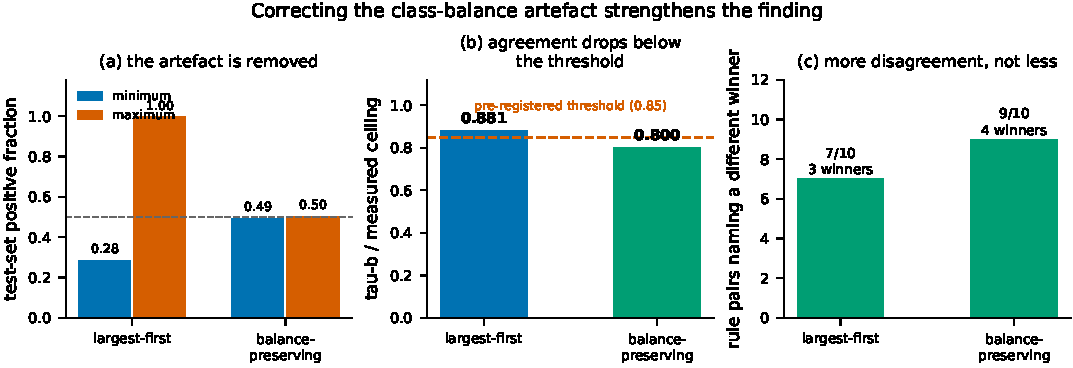
\includegraphics[width=\textwidth]{F8_balanced_comparison.pdf}
\caption{Correcting the class-balance artefact removes it entirely and strengthens, rather
than weakens, the ranking finding.}
\label{fig:balanced}
\end{figure}

\subsubsection*{(c) It induces covariate shift, sometimes reversing a feature}

Held-out clusters are by construction the sequences least similar to the training set, so
the held-out partition can differ systematically in exactly the features a model relies on.
Net-charge separation between classes shifts from $+1.80$ (train) to $\mathbf{-1.48}$
(test) in toxicity and from $+1.18$ to $-0.12$ in antifungal: \textbf{the relationship
between charge and the label inverts between partitions}. Positive-class median length
shifts by up to 40 residues. The shift is associated with apparent difficulty
(Spearman $\rho = -0.624$, $p = 0.054$ for charge-gap loss; $\rho = -0.564$, $p = 0.090$
for composition shift); with ten tasks these are suggestive rather than established, though
the sign reversals are directly observable.

\begin{figure}[htbp]\centering
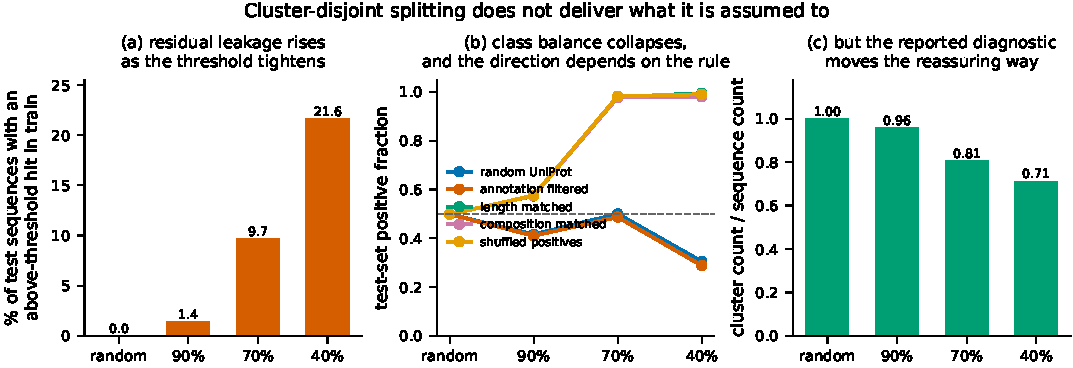
\includegraphics[width=\textwidth]{F7_splitting_artefacts.pdf}
\caption{Three artefacts of cluster-disjoint splitting. The diagnostic a benchmark would
naturally report (panel c) moves in the opposite direction to both problems.}
\label{fig:artefacts}
\end{figure}

\subsubsection*{(d) Published benchmarks contain exact duplicates across their own splits}

Of the 16 datasets in the collection, \textbf{11 contain sequences present in both
partitions}, listed in full in Supplementary Table~S3. These are byte-identical
strings, which any similarity threshold must treat as 100\% identical; we remove the
test-side copy before scoring and report the count. Separately, sequences appear
\emph{with both labels} inside a single partition, most heavily in antibacterial (295 in
train, 31 in test).


\paragraph{Which splits were used for the reported runs.} Arm~A uses each dataset's
\emph{released} \texttt{train.csv}/\texttt{test.csv} partition unchanged, with the
test-side copy of any cross-split duplicate dropped before scoring and no other
modification; the five seeds vary model initialisation and data order, not the partition,
which is fixed by the publisher. Arm~B generates its own partitions, and every Arm~B number
is reported under one of two named splitters (largest-first or balance-preserving,
Table~\ref{tab:definitions}), never a mixture.

We note these neutrally. They are observations about released files, and they were only
checkable because the authors released them. The point is not that this collection is
careless -- it is unusually careful, and the duplicates survived anyway.

%=======================================================================
\section{Uncertainty, and a direct test of the two arms}
%=======================================================================

\subsection{Headline statistics with intervals}

The point estimates, ceilings and normalised values for all four statistics are given once,
in Table~\ref{tab:definitions}, and are not repeated here. This section adds the
uncertainty: Table~\ref{tab:leveljack} below carries both kinds of interval side by side,
computed in one run of each estimator (3{,}000 resamples for the pipeline bootstrap, ranks
recomputed inside each resample).

Marginal top-1 flip rates, computed on seed-averaged scores, are $0.933$ $[0.800, 0.956]$
in Arm~A over 45 pairs and $0.900$ $[0.400, 0.900]$ in Arm~B over only ten; both intervals
resample pairs and are therefore anticonservative, and the Arm~B one is too wide to support
a conclusion on its own. Sections~\ref{sec:flip-ceiling}
and~\ref{sec:level-uncertainty} replace both with a matched contrast against a measured
ceiling and with level-based intervals.

\subsection{The flip rate against its own ceiling}
\label{sec:flip-ceiling}

Section~\ref{sec:tau-protocol} insists that $\tau_b$ be read against a measured ceiling
rather than against $1.0$. The same argument applies to the flip rate, and applying it is
the sharper test: reseeding alone reorders near-tied pipelines, so some winner changes are
run noise rather than protocol sensitivity. Quoting a flip rate against an implicit floor
of zero makes exactly the mistake the ceiling was introduced to prevent.

We therefore measure the ceiling the same way, and make the contrast matched on seed --
across levels with the seed held fixed, against across seeds with the level held fixed.
Averaging over seeds before taking the winner, as the marginal flip rates above do,
suppresses run noise in the first term but not the second, so the two would not otherwise
be comparable.

\begin{table}[htbp]\centering\small
\caption{Top-1 flip rate against its measured seed-noise ceiling, matched on seed.
\emph{Normalised excess} is $(\text{observed} - \text{ceiling})/(1 - \text{ceiling})$: the
share of the room above the noise floor that the factor actually uses. Bootstrap over
pairs, 20{,}000 resamples.}
\label{tab:flipceiling}
\begin{tabular}{llrrcr}
\toprule
Factor varied & arm & flip & ceiling & difference (95\% CI) & norm.\ excess \\
\midrule
biological task      & A & 0.933 & 0.570 & ${+}0.363$ $[{+}0.262, {+}0.467]$ & \textbf{0.845} \\
negative-set rule    & B & 0.760 & 0.545 & ${+}0.215$ $[{+}0.125, {+}0.305]$ & 0.473 \\
clustering threshold & B & 0.753 & 0.545 & ${+}0.208$ $[{+}0.110, {+}0.305]$ & 0.458 \\
negative-set rule\textsuperscript{$\ddagger$} & B & 0.730 & 0.585 & ${+}0.145$ $[{+}0.055, {+}0.235]$ & 0.349 \\
\bottomrule
\end{tabular}

\vspace{2pt}
\footnotesize\raggedright
\textsuperscript{$\ddagger$}Under the pre-registered splitter; the three rows above use the
balance-preserving splitter. All four differences have $p \leq 0.002$.
\end{table}

Three things follow, and the first is a correction to our own emphasis.

\textbf{The winner is unstable even to reseeding.} The ceiling is $0.545$ in Arm~B and
$0.570$ in Arm~A: \emph{more than half} of all winner changes are reproduced by changing
nothing but the random seed. A benchmark that reports a single run and names a best method
is, on this evidence, reporting a coin flip about as often as not. This is a stronger
practical warning than anything we had framed as a headline, and it is independent of
protocol choice entirely.

\textbf{Within these levels, protocol choice flips the winner more often than noise does --
but this is descriptive, not an inference about protocols in general.} Every factor exceeds
its ceiling in the table above, and the pre-registered splitter still shows an excess
(${+}0.145$, $[{+}0.055, {+}0.235]$), so the pattern does not depend on the post hoc
correction of Section~\ref{sec:artefacts}. We nevertheless decline to call the Arm~B
version significant, for a reason that is structural rather than cautious: \textbf{the
intervals in Table~\ref{tab:flipceiling} resample pairs, and the ten rule pairs are built
from only five rules}, each appearing in four pairs. They are not independent evidence, so
a bootstrap over pairs understates uncertainty. Resampling the rules themselves gives a
level-based interval on B1's flip rate of $[0.060, 1.000]$
(Section~\ref{sec:level-uncertainty}) -- five levels cannot locate that rate at all.

So we make two claims of different strength. \emph{For these five negative-set rules}, the
winner changes in most pairs and more often than reseeding alone changes it: that is a
measurement, and it is the experience of a practitioner switching between two published
negative-set definitions. \emph{For negative-set rules in general}, we make no claim; the
data do not support one and we have not smuggled it in through a $p$-value computed over
pairs.

\textbf{Task variation again dominates, and there the claim does generalise.} Changing the
biological question consumes $84.5\%$ of the available room above the noise floor, against
$47.3\%$ for the negative-set rule. With ten tasks rather than five rules the level-based
interval on the task flip rate is $[0.853, 1.000]$, so unlike Arm~B this one survives
resampling of the levels -- still within the one curated collection those ten tasks come
from.

\subsection{The two arms differ, and task variation is the larger effect}

Both arms rank the same pipelines, so the comparison is paired at the pipeline level: we
resample pipelines once per iteration and recompute \emph{both} $\tau_b$ values on that
same resample. A permutation test swapping rows between arms is unavailable, since the arms
have ten and five levels respectively and the rows are not exchangeable; we attempted it,
it failed on the dimension mismatch, and we replaced it rather than forcing a test the data
do not support.

\begin{center}\small
\begin{tabular}{lcc}
\toprule
Arm~B splitter & pre-registered & balance-preserving \\
\midrule
$\tau_b$, varying protocol                & 0.727 & 0.693 \\
$\tau_b$, varying task (shared pipelines) & 0.508 & 0.508 \\
\textbf{difference}                       & $\mathbf{+0.218}$ & $\mathbf{+0.185}$ \\
95\% CI                                   & $[+0.117,\ +0.317]$ & $[+0.110,\ +0.269]$ \\
two-sided $p$                             & $0.001$ & $0.00025$ \\
\bottomrule
\end{tabular}
\end{center}

\noindent\textbf{Across these five rules and ten tasks, changing the biological task
disturbs the ranking more than changing the evaluation protocol.} Neither arm alone could
have established this.

Two qualifications belong with that sentence rather than in a limitations list. First, the
intervals above resample pipelines and so hold the levels fixed; generalised over levels the
difference is ${+}0.218$ $[{+}0.029, {+}0.408]$, $p = 0.024$ under the primary analysis
\textbf{B1} and ${+}0.185$ $[{-}0.061, {+}0.431]$, $p = 0.141$ under the post hoc
\textbf{B2} (Section~\ref{sec:level-uncertainty}). The claim rests on B1. Second, Arm~A
varies the biological question and not the curator, so this contrasts \emph{tasks within a
protocol} (Section~\ref{sec:canclaim}).

\subsection{Cluster-aware intervals on the scores}
\label{sec:cluster-ci}

The intervals above are all on rank statistics. The scores have their own
uncertainty, and the usual sequence-level bootstrap is optimistic for peptides because test
sequences are related to one another and are therefore not independent draws. We recomputed
key score intervals resampling whole similarity clusters instead, which requires refitting
with the predictions retained -- the stored run records hold aggregate metrics only -- so we
scoped it to the five negative rules at threshold $0.7$ (16 pipelines) and the five smallest
Arm~A tasks (24 pipelines), the latter being where a sequence-level interval is most
optimistic. For Arm~B the resampling unit is the same clustering that defined the split; for
Arm~A, which ships a partition with no published clustering, the test set is clustered at
40\% identity, the coarse end, chosen because coarser clusters give wider intervals.


\begin{figure}[htbp]\centering
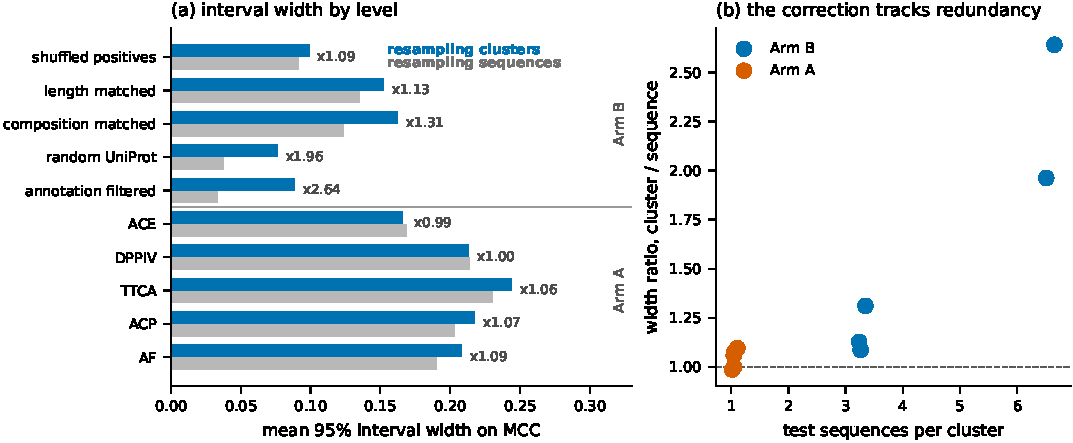
\includegraphics[width=\textwidth]{F12_cluster_intervals.pdf}
\caption{(a) Mean 95\% interval width on MCC, resampling test sequences against resampling
whole similarity clusters, with the ratio beside each pair. (b) The size of the correction
is explained by one quantity: how many test sequences share a cluster. Arm~B's
proteome-derived rules carry $6.5$--$6.7$ sequences per cluster and need the largest
correction; Arm~A's native partitions are near-singletons and need essentially none.}
\label{fig:clusterci}
\end{figure}

\textbf{In Arm~B the sequence-level interval is too narrow, by $1.63\times$ on average and
$2.64\times$ at worst} (Figure~\ref{fig:clusterci}), and the correction is largest for
annotation-filtered and random
UniProt. The mechanism is visible in the table: whole proteome sequences form families, so
those test partitions hold $6.5$--$6.7$ sequences per cluster, while negatives synthesised
from the positives are near-singletons at $3.2$--$3.3$. The two rules whose test sets are
most internally redundant are once again the two that look easiest and that carry the
provenance asymmetry of Section~\ref{sec:exposure} -- three separate reasons to distrust a
high score obtained that way, all pointing at the same two rules.

\textbf{In Arm~A the correction is negligible}, ratio $1.04$, and this is a point in the
curated collection's favour that we want to state as plainly as we have stated its
duplicates. At 40\% identity its test partitions are essentially sets of singletons
($1.0$--$1.1$ sequences per cluster), so a sequence-level interval is already adequate there
and the homology-aware partitioning did what it was meant to do within the test set. Not
every diagnostic in this paper finds a problem.

\textbf{What the small tasks cannot do, however, is identify a winner.} In all five, the
best pipeline's 95\% cluster interval overlaps that of the \emph{median} pipeline of 24 --
for example on tumour T-cell antigen the best scores MCC $0.771$ $[0.667, 0.867]$ against
the median's $0.630$ $[0.503, 0.754]$, and on anticancer $0.327$ $[0.220, 0.427]$ against
$0.267$ $[0.155, 0.371]$. The overlap holds under the sequence bootstrap too, so it is not
an artefact of the cluster correction: these test sets are simply too small to separate the
top of the leaderboard from its middle. That is an independent route to the same conclusion
as Section~\ref{sec:flip-ceiling} -- winner identity is the fragile quantity -- reached
without any rank statistic, and it explains why rank transfer across small tasks is poor
whatever the protocol.

\subsection{Generalising over levels, not just over pipelines}
\label{sec:level-uncertainty}

Every interval so far resamples pipelines and therefore holds the five rules and ten tasks
fixed (Section~\ref{sec:definitions}). Our headline claims are about protocols and tasks, so
Table~\ref{tab:leveljack} recomputes them with the delete-one-level jackknife. The
intervals roughly double in width, and for the flip rate they become close to
uninformative.

\begin{table}[htbp]\centering\small
\caption{Delete-one-level jackknife intervals, which generalise over the \emph{level}
population, beside the pipeline-resampling intervals reported earlier. With four to ten
levels these are necessarily wide; that width is the honest precision of a claim about
protocols or tasks in general.}
\label{tab:leveljack}
\begin{tabular}{llcccc}
\toprule
 & & \multicolumn{2}{c}{mean $\tau_b$, 95\% CI} & \multicolumn{2}{c}{top-1 flip rate, 95\% CI} \\
\cmidrule(lr){3-4}\cmidrule(lr){5-6}
Label & levels & resampling pipelines & \textbf{level jackknife} & resampling pairs & \textbf{level jackknife} \\
\midrule
\textbf{B1} & 5 rules      & $[0.609,\ 0.818]$ & $[0.561,\ 0.893]$ & $[0.400,\ 0.900]$ & $[0.060,\ 1.000]$ \\
B2 & 5 rules      & $[0.586,\ 0.769]$ & $[0.465,\ 0.922]$ & $[0.400,\ 0.900]$ & $[0.580,\ 1.000]$ \\
B3 & 4 thresholds & ---               & $[0.824,\ 0.954]$ & ---               & $[0.000,\ 1.000]$ \\
A1 & 10 tasks     & $[0.351,\ 0.564]$ & $[0.395,\ 0.563]$ & $[0.800,\ 0.956]$ & $[0.853,\ 1.000]$ \\
\bottomrule
\end{tabular}
\end{table}

Three consequences, and we state the uncomfortable one first.

\textbf{The winner-flip rate does not support a population claim in Arm~B.} At five rules
the level-jackknife interval on B1's flip rate is $[0.060, 1.000]$. The observation that
most rule pairs crown a different pipeline is solid \emph{for these five rules}, and it is
the experience a practitioner has when switching between two published negative-set
definitions; but five levels cannot locate that rate in a wider population. In Arm~A, with
ten tasks, the interval is $[0.853, 1.000]$ and the claim does survive generalisation.

\textbf{Arm~A's agreement is the better-determined of the two}, because ten levels beat
five: its two intervals nearly coincide ($[0.351, 0.564]$ against $[0.395, 0.563]$),
whereas B2's widens from $[0.586, 0.769]$ to $[0.465, 0.922]$.

\textbf{The two-arm difference survives under the primary analysis and not under the post
hoc one.} Treating the rule set and the task set as independent samples of levels, the
jackknife standard error of the difference is $\sqrt{\mathrm{SE}_B^2 + \mathrm{SE}_A^2}$:

\begin{center}\small
\begin{tabular}{lcc}
\toprule
Arm~B splitter & \textbf{B1} pre-registered \emph{(primary)} & B2 balance-preserving \emph{(post hoc)} \\
\midrule
difference in $\tau_b$                  & $+0.218$ & $+0.185$ \\
level-jackknife SE                      & $0.097$  & $0.126$ \\
95\% CI, generalising over levels       & $[+0.029,\ +0.408]$ & $[-0.061,\ +0.431]$ \\
two-sided $p$                           & $\mathbf{0.024}$ & $0.141$ \\
\midrule
95\% CI, resampling pipelines only      & $[+0.117,\ +0.317]$ & $[+0.110,\ +0.269]$ \\
\bottomrule
\end{tabular}
\end{center}

\noindent Under B1, the pre-registered and primary comparison, task variation disturbs the
ranking significantly more than protocol variation even when the inference is generalised
over levels ($p = 0.024$). Under B2 it does not ($p = 0.141$), because correcting the
class-balance artefact lowers Arm~B's agreement toward Arm~A's and simultaneously widens
its level-jackknife interval. \textbf{The claim therefore stands on the primary analysis
and is weakened, not strengthened, by the post hoc correction} -- the opposite of the
direction a reader might suspect a post hoc analysis of being chosen for, and we flag it
rather than reporting only the favourable pairing. Because the sign agrees in both and the
primary is significant, we retain the claim, restricted to these five rules and ten tasks.

\subsection{Design-simulation limits, pre-specified}

Before any data were analysed we characterised the estimator. The mean of pairwise $\tau_b$
has null SD $0.069$ at 12 pipelines and 5 protocols, against $0.219$ for a single pair;
minimum detectable disagreement at 80\% power is $\tau_b \leq 0.646$ at 16--20 pipelines,
which is why a pre-registered observation of $0.727$ was reported as inconclusive rather
than as a near-miss. The simulation assumed a ceiling of $0.955$ at 5\% run noise; the
\emph{measured} ceilings were $0.867$ (Arm~B) and $0.838$ (Arm~A), so real run-to-run noise
is larger than assumed and the simulation was, if anything, optimistic
(Supplementary Figure~S2).


%=======================================================================
\section{Discussion}
%=======================================================================

\subsection{What this study can and cannot settle}
\label{sec:canclaim}

Before any interpretation, the boundary of the evidence, because every claim below sits
inside it and the reader should not have to reach the limitations section to find out.

\textbf{Arm~B varies five negative-set construction rules around one fixed positive set of
5{,}187 peptides.} The positive set is ours to the extent that we chose which published
collection to build on; the five rules span the families behind eleven published definitions
but are not those eleven implementations. Conclusions attach to these five rules on this
corpus.

\textbf{Arm~A varies ten biological tasks that come from a single collection, curated by
one group with one homology-aware partitioning pipeline}~\citep{fernandezdiaz2024autopeptideml}.
This is the limitation that most constrains the paper's reach. Those ten datasets share a
curator, a label convention, a negative-set philosophy and a splitting procedure. What
varies between them is the biological question; what does \emph{not} vary is everything
about how the benchmark was built. Arm~A therefore measures \textbf{task transfer under a
fixed protocol}, and it is not a cross-benchmark comparison in any form.

\textbf{We did not compare independently constructed benchmarks.} That was the original
motivation and it remains open (Section~\ref{sec:prereg}, deviation 1). Nothing here is
evidence that independently built benchmarks agree or disagree, and a reader who wants that
question answered should treat this paper as instrumentation and a set of measured
artefacts rather than as the answer. Settling it needs several genuinely independent
resources harmonised to a common task definition and each reproduced to its own published
baseline -- the gate we pre-specified and could not apply.

\textbf{The honest size of the contribution}, then: a decomposition showing which design
choice owns the reported number, four measured failures of a splitting method the field has
standardised on, two agreement statistics reported against measured ceilings instead of
nominal maxima, and a pre-registered null. All of it demonstrated on one corpus and one
curated task collection.

\subsection{What we set out to test, and what we found instead}

We pre-registered the hypothesis that leakage-controlled evaluation protocols would rank a
fixed set of methods differently, and fixed the decision thresholds in advance. Under the
pre-registered analysis \textbf{that hypothesis was not supported}: normalised agreement
was $0.881$ against a threshold of $0.85$, and $\tau_b = 0.727$ fell inside the band we
had declared inconclusive for this design. Had we not fixed those thresholds in advance,
$0.727$ would have been straightforward to present as disagreement.

Because the result was a null, the interesting question became why the intuition was
wrong, and in what narrower sense it is right.

\subsection{The ordering is stable; the winner is not}

Two facts must be held together: mean $\tau_b$ across protocols is high, and 9 of 10
protocol pairs name a different best pipeline. These are not in tension. $\tau_b$ weights
all pairwise orderings equally, and most are stable -- the weakest pipelines occupy the
bottom places under every protocol, contributing concordant pairs regardless. The
reordering concentrates among the leading pipelines, which are close in score and therefore
easy to permute. \textbf{A rank correlation computed over a whole leaderboard is the wrong
instrument for a field that reads only the top of it.}

That the leading places are close enough to permute easily has a consequence we did not
anticipate and that cuts against our own framing. If the top pipelines are separated by
less than run-to-run noise, then the seed alone should move the winner -- and it does, in
$54.5\%$ of comparisons (Section~\ref{sec:flip-ceiling}). Protocol choice flips the winner
more often than that, in $76.0\%$ of comparisons, and the excess appears under both
splitters -- though with five rules we report it as a measurement on those rules rather
than as an inference about protocols, since resampling the rules leaves the rate
undetermined. But the honest summary is two-part: \textbf{the winner is
a noisy statistic before any protocol is varied, and varying the protocol makes it
substantially noisier}. The practical recommendation that follows is not only to report
rankings under a second negative-set rule, but to report the winner's stability across
seeds at all -- which almost no benchmark currently does, and which costs five reruns.

\subsection{Protocol moves the score; interaction moves the rank}

The negative-set rule accounts for $71.0\%$ of the variance in MCC, against $14.8\%$ for
the pipeline and $0.6\%$ for the clustering threshold. The single largest determinant of a
reported number in this literature is a construction choice that has no standard and is
often described in one sentence.

Protocol main effects contribute \emph{nothing} to rank variance, but we want to be exact
about why, because we initially presented this as a finding and it is not one. Ranks are
computed within each protocol cell, so every cell's mean rank is $(K+1)/2$ by construction
and any cell-defining factor has zero between-group sum of squares identically, for any
data (Section~\ref{sec:structural-zero}). The useful content of the rank decomposition is
in the interactions, which are free to vary: pipeline $\times$ rule is $8.87\%$
$[8.30, 9.43]$, seven times pipeline $\times$ threshold at $1.26\%$ $[0.97, 1.55]$.

We still recommend decomposing both responses, with the caveat made explicit: when a paper
claims a design factor matters, ask whether it matters to the number or to the conclusion
drawn from the number -- but read a zero on the rank response as a property of the
estimator unless the factor is nested rather than crossed with the ranking unit.

\subsection{Task transfer is the larger problem}

Rank agreement is lower across biological tasks than across evaluation
protocols. Generalising over levels, which is the population the claim is about, the
difference is ${+}0.218$ $[{+}0.029, {+}0.408]$, $p = 0.024$ under the pre-registered
splitter and ${+}0.185$ $[{-}0.061, {+}0.431]$, $p = 0.141$ under the post hoc one; holding
the levels fixed and resampling only pipelines gives ${+}0.218$ $[{+}0.117, {+}0.317]$,
$p = 0.001$ and ${+}0.185$ $[{+}0.110, {+}0.269]$, $p < 0.001$ respectively. The claim
rests on the pre-registered splitter, and on these ten tasks and five rules
(Section~\ref{sec:canclaim}).

Seven different pipelines win across ten tasks and one moves 20 of 24 positions. The field has invested
heavily in standardising the splitting protocol -- the factor our data identify as the
\emph{smaller} of the two -- and has no convention at all for either the negative-set rule
or for reporting whether a method's advantage transfers beyond the task it was demonstrated
on.

\subsection{Four artefacts of a method the field has standardised on}

Cluster-disjoint splitting does not deliver what it is assumed to. It is not
pairwise-disjoint, and residual leakage \emph{rises} with nominal strictness, reaching
$21.6\%$ overall and $39\%$ for whole-protein negatives. It destroys class balance, up to
$99.5\%$ positive on a 1:1 corpus. It induces covariate shift that in two tasks reverses
the sign of a discriminative feature. And the diagnostic a benchmark would naturally
report -- the cluster-to-sequence ratio -- moves reassuringly in the opposite direction to
all of these.

None of this is an argument against homology-aware splitting; random splitting is plainly
worse. It is an argument that the residual is large, systematic, largest where the claim
sounds strongest, and currently unreported.

\subsection{What is confirmatory, what is post hoc, and what is an observation}
\label{sec:status}

The strongest sentences in this paper are not the best-supported ones, and a reader is
entitled to see that sorted out explicitly rather than inferred from hedging. Only one
result is confirmatory, and it is a null.

\begin{table}[htbp]\centering\small
\caption{Evidential status of every claim we make. \emph{Confirmatory} means tested against
a threshold fixed before the data were analysed. \emph{Post hoc} means the analysis was
designed after seeing results. \emph{Descriptive} means a measurement on these specific
corpora with no inferential claim attached, which is where our rhetorically strongest
observations sit.}
\label{tab:status}
\footnotesize
\begin{tabular}{>{\raggedright\arraybackslash}p{0.50\textwidth}%
                >{\raggedright\arraybackslash}p{0.23\textwidth}%
                >{\raggedright\arraybackslash}p{0.16\textwidth}}
\toprule
Claim & Status & Generalises to \\
\midrule
H1: protocols rank methods differently (\textbf{B1}, normalised $0.881$ vs threshold
  $0.85$) -- \textbf{not supported} & confirmatory & these 5 rules \\
\addlinespace
Task variation disturbs ranking more than protocol variation
  (${+}0.218$, $p = 0.024$ over levels) & secondary, pre-specified estimator
  & these 5 rules, 10 tasks \\
\addlinespace
Negative-set rule owns $71.0\%$ of score variance vs pipeline $14.8\%$ (H3)
  & secondary, pre-specified & this corpus \\
Seed component negligible (H4) & secondary, pre-specified & this corpus \\
\addlinespace
Winner flips above its seed-noise ceiling, \emph{across tasks} ($0.933$ vs $0.570$;
  level-based CI $[0.853, 1.000]$) & post hoc (ceiling added after an audit of our own
  reasoning) & these 10 tasks \\
Winner flips above its seed-noise ceiling, \emph{across negative-set rules} ($0.760$ vs
  $0.545$; level-based CI $[0.060, 1.000]$) & post hoc, \textbf{descriptive only} -- five
  levels cannot locate the rate & these 5 rules \\
Balance-preserving splitter lowers agreement to $0.800$ (\textbf{B2})
  & post hoc & this corpus \\
\addlinespace
Residual pairwise leakage rises as the threshold tightens ($1.4\% \to 21.6\%$)
  & descriptive & this corpus \\
Cluster-disjoint splitting destroys class balance (to $99.5\%$ positive)
  & descriptive & this corpus \\
Covariate shift inverts a feature's sign in 2 tasks & descriptive & those 2 tasks \\
11 of 16 released datasets contain cross-split duplicates & descriptive, verifiable
  & that collection \\
Two-feature baseline reaches MCC $0.79$ on proteome negatives & descriptive & this corpus \\
\addlinespace
``The field has standardised the factor that matters less to the ranking''
  & interpretation & -- \\
\bottomrule
\end{tabular}
\end{table}

The last row deserves naming for what it is. Statements about what ``the field'' has
standardised, and about what benchmark results mean in general, are \textbf{interpretation}:
they are our reading of why the measured pattern matters, not findings. We have kept them
because we think they are the right reading and because a paper that refuses to interpret
its own results is less useful, not more rigorous. But they are not evidence, they are not
pre-specified, and nothing in Table~\ref{tab:status} above them depends on accepting them.

\subsection{Limitations}

\begin{itemize}[leftmargin=1.4em,itemsep=2pt]
\item \textbf{Scope: five rules on one corpus, ten tasks from one curator.} Stated in full
  in Section~\ref{sec:canclaim} and not restated here. In short: Arm~B's corpus is ours and
  is instrumentation rather than a proposed standard; Arm~A varies the biological question
  at a fixed protocol; the cross-benchmark comparison was not performed and remains open.
\item \textbf{The balanced splitter is post hoc.} It was built after the pre-registered
  null. We report it as a sensitivity analysis and do not claim it confirms the hypothesis.
\item \textbf{The RBF SVM is approximated} by a Nystr\"om map -- the one substitution that
  changes a model rather than its scheduling. We validated it against the exact kernel on 15
  matched cells (Section~\ref{sec:svm-validation}): it costs about 0.03--0.04 of AUROC and
  MCC but preserves the rule-level ordering ($r = 0.997$ on MCC). The approximation lowers
  one pipeline's absolute scores; it does not move the rankings this paper reports.
\item \textbf{CPU-only hardware excluded two pipeline families} -- end-to-end convolutional
  and recurrent models, and a 3B-parameter language model -- so we cannot say whether
  end-to-end sequence models are more or less protocol-sensitive.
\item \textbf{Covariate-shift correlations are marginal} at ten tasks
  ($p = 0.054$, $p = 0.090$) and are reported as suggestive.
\item \textbf{H1 was pre-specified, not registered.} The analysis plan is dated and
  released but was not externally deposited, and its primary hypothesis originally named
  five published benchmarks as the comparison unit rather than the protocol levels we
  ultimately varied (Section~\ref{sec:prereg}, deviation 1). A reader should discount H1's
  confirmatory status accordingly.
\item \textbf{The rank-variance decomposition cannot speak to protocol main effects.}
  They are zero by construction, not by measurement (Section~\ref{sec:structural-zero}).
  Our evidence that protocol preserves ordering is the rank-agreement and flip-rate
  analyses, not the decomposition.
\item \textbf{Class provenance is asymmetric, and we did not test pretraining exposure.}
  Under the two proteome-derived rules every negative and $7.9\%$ of positives are verbatim
  reviewed-UniProt entries (Section~\ref{sec:exposure}). That is an overlap audit against
  the \emph{current} release; ESM-2 was trained on UniRef from release 2021\_04, so our
  audit bounds exposure in neither direction, and we do not claim it does. Whether the
  encoder had seen these sequences remains untested.
\item \textbf{The negative realisation was fixed per rule in the main grid.} A single draw
  per rule was embedded, because embedding five draws at four ESM-2 scales was not
  affordable on CPU, so the reported seed component varies the partition and model
  initialisation but \emph{not} which negatives were sampled. We quantify draw-to-draw
  variability separately on the embedding-free pipelines
  (Section~\ref{sec:draw}): the rule dominates the draw about two to one, but for the two
  matched-negative rules the draw alone moves the ranking to normalised $0.65$--$0.69$, so
  their variance components are conditional on the realisation rather than marginal over it.
\end{itemize}

\subsection{Recommendations}

In order of value per unit of effort.

\begin{enumerate}[leftmargin=1.6em,itemsep=2pt]
\item \textbf{Measure and publish residual pairwise leakage.} Search the test partition
  against the training partition and report the fraction of test sequences with an
  above-threshold hit. Cluster-disjointness does not imply it, and it costs one search.
\item \textbf{Report test-set class balance per split.} It is one number and it can be
  $0.99$ without anyone noticing.
\item \textbf{Rerun with five seeds and report whether the winner survives.} In our grids
  reseeding alone changes the top-ranked pipeline in $54.5\%$ of comparisons
  (Section~\ref{sec:flip-ceiling}). A leaderboard that names a best method from one run is
  reporting a statistic it has not shown to be stable, and the check costs five fits.
\item \textbf{Include a trivial baseline.} Length and net charge cost nothing. If two
  features place near the top, fix the negative set before publishing the model.
\item \textbf{Report rankings under at least two negative-set rules}, and state whether a
  method's advantage transfers to a second task.
\item \textbf{Quote agreement against a measured ceiling, not against $1.0$.} Seed
  replicates give the ceiling free; ours were $0.838$ and $0.867$.
\item \textbf{Report the metric you chose and the ranking under alternatives.}
\item \textbf{Assign clusters in random order, not by size.} Size-ordered assignment is what
  produces both the class-balance collapse and the worst residual leakage; a uniform shuffle
  of cluster order cut mean leakage from $0.107$ to $0.055$ and balance error from $0.305$ to
  $0.009$ in our stress test, and costs one line (Table~\ref{tab:stresstest}). If leakage
  matters more than balance, order by how little each cluster bridges to the rest.
\item \textbf{Publish split files, not split procedures}, and state the clustering tool,
  threshold \emph{and} coverage parameter. For matched-negative rules, publish the
  \emph{realisation} too: redrawing the negatives under a fixed rule moved our rankings to
  normalised $0.65$--$0.69$ (Section~\ref{sec:draw}), so the rule alone does not specify the
  benchmark.
\item \textbf{Check for exact duplicates across your own split.} Eleven of sixteen
  carefully built datasets contained them.
\end{enumerate}

\subsection{Conclusion}

Homology-aware splitting corrected a real problem and the field is better for it. It did
not make evaluation interchangeable across the levels we varied, but the failure is more
specific than expected and more actionable for it. Protocol choice does not scramble the
ranking of methods -- the broad ordering is largely preserved, retaining $88\%$ of the
agreement that rerunning the same protocol achieves -- while it changes which method is
crowned in 9 of 10 rule pairs, and it changes the apparent difficulty of the task by
$0.6$ MCC. Varying the biological question disturbs the ranking more still. Since the
literature advances by adopting whatever placed first, those are the failures that matter.

All of it holds for \textbf{five negative-set rules on one corpus} and \textbf{ten tasks
from one curator}, the boundary set out in Section~\ref{sec:canclaim}. Within those levels
the effects are large and measured; generalised beyond them our own intervals are wide
enough that we decline to make the claim.

The splitting method itself needs attention independently: as standardly implemented it
leaves up to $21.6\%$ of the test set leaking at its strictest setting, can return a test
partition that is $99.5\%$ one class, and can invert the sign of the very feature a model
depends on -- while the statistic a benchmark would report to reassure a reader moves in
the opposite direction to all three.

%=======================================================================
\section*{Data and code availability}
%=======================================================================

All analysis code, the frozen pipeline specification, the protocol configuration, the
complete record of all model fits and the scripts that regenerate every figure and table
are released as a single archive, \texttt{bra-harness.tar.gz}, with SHA-256\\
\texttt{e43629198237357d4412a2a28740da0829c4cdea}\-\texttt{aae34263848889ffad608f35}\\
\textbf{Deposit URL/DOI: \textcolor{red}{INSERT\_AT\_DEPOSIT}}.

The dated analysis plan, including all three revisions and the complete deviations log
discussed in Section~\ref{sec:prereg}, is released in the archive as
\texttt{preregistration.md}. It was not deposited with an external registry and carries no
third-party timestamp; we say so there as well as here.

\texttt{reproduce.sh} reruns the study end to end from a clean checkout, including input
retrieval, and is idempotent and resumable at both the embedding stage (cache keyed by
sequence hash) and the grid stage (one file per cell).

The Arm~B corpus is not redistributed: its positives derive from DBAASP via the
AMPBenchmark positive set and its negatives from UniProt, and those terms govern
redistribution. We release the construction scripts with SHA-256 hashes of both inputs,
which reconstructs the corpus given the same source files. The Arm~A datasets are
redistributed by their original authors and are not duplicated here.

\paragraph{What the released run records cover.} ``4{,}400 run records'' refers to the two
main factorial designs and nothing else. The supplementary analyses add 530 further model
fits and are deposited in the same archive, each with the script that produced it and the
table it writes.


\paragraph{Exact inputs needed to rebuild the corpora.} Reproduction depends on pinned
inputs, not just on pinned code, so we state each one and how it is verified:

\begin{itemize}[leftmargin=1.4em,itemsep=2pt]
\item \textbf{Arm~B positives} -- the published positive set of
  \citet{sidorczuk2022negative} (AMPBenchmark), SHA-256 recorded in the archive. 5{,}187
  sequences after removing the three homopolymers named in the Methods.
\item \textbf{Arm~B negatives} -- reviewed UniProt (SwissProt), \textbf{retrieved
  2026-10-05}, 575{,}749 records of which 573{,}063 are fully canonical. Because UniProt
  releases are not immutable at a stable URL, the archive records the SHA-256 of the
  retrieved FASTA; rebuilding against a later release will not reproduce the corpus
  byte-for-byte, and \texttt{reproduce.sh} fails loudly on a hash mismatch rather than
  proceeding with different negatives.
\item \textbf{Arm~A datasets} -- the AutoPeptideML peptide benchmark collection
  \citep{fernandezdiaz2024autopeptideml}, 16 datasets, used as released; per-dataset row
  counts and SHA-256 values are in the archive, and the sizes are printed in
  Supplementary Table~S3 so a reader can check a download without running anything.
\item \textbf{Tools} -- MMseqs2 18-8cc5c+ds-1 and the Python versions listed above; the
  clustering call is given in full in the Methods, coverage parameter included.
\end{itemize}

\paragraph{Status of the deposit.} \textcolor{red}{The archive hash above is final and the
deposit identifier must be inserted before submission.} We flag this rather than leave it
implicit: a reproducibility claim with no resolvable location is not a claim a reader can
act on, so until the DOI is present the availability statement should be read as an
undertaking rather than as a completed deposit.

Software: Python 3.12.15, numpy 2.5.3, pandas 3.0.6, scipy 1.18.1, scikit-learn 1.9.1,
XGBoost 3.4.1, PyTorch 2.14.1 (CPU), MMseqs2 18-8cc5c+ds-1, qmap-benchmark 0.1.1.
Reference hardware: AMD Ryzen 9 8940HX, 32 threads, no GPU.

%=======================================================================
\section*{Acknowledgements}
%=======================================================================

We thank the authors of AMPBenchmark, whose published positive set and negative-sampling
definitions underlie Arm~B, and of AutoPeptideML, whose curated task collection and native
homology-aware partitions constitute Arm~A. We also thank the authors of QMAP, PPB and
GenPept-Curated-2025, whose resources informed the design even where they do not appear in
the executed grids. This study was only possible because all of them released data, code
and protocols openly, and our findings about evaluation practice are not criticisms of
their work: every benchmark we examined controls homology more carefully than the
literature it improved upon, and the duplicate counts we report were only checkable
because the files were published at all.

\section*{Conflicts of interest}
None declared.

%=======================================================================
%  Bibliography, embedded. BibTeX is not required.
%  Order follows first citation, matching the unsrtnat style.
%=======================================================================
\begin{thebibliography}{22}

\bibitem[{Sidorczuk et~al.}(2022)]{sidorczuk2022negative}
K.~Sidorczuk, P.~Gagat, F.~Pietluch, J.~Kala, D.~Erbert, and M.~Burdukiewicz.
\newblock Benchmarks in antimicrobial peptide prediction are biased due to the selection
  of negative data.
\newblock \emph{Briefings in Bioinformatics}, 23(5):bbac343, 2022.

\bibitem[{Fern\'andez-D\'iaz et~al.}(2024)]{fernandezdiaz2024autopeptideml}
R.~Fern\'andez-D\'iaz, R.~Cossio-P\'erez, C.~Agoni, H.~T. Lam, V.~Lopez, and D.~C. Shields.
\newblock {AutoPeptideML}: a study on how to build more trustworthy peptide bioactivity
  predictors.
\newblock \emph{Bioinformatics}, 40(9):btae555, 2024.

\bibitem[{Ferrer Florensa et~al.}(2024)]{ferrerflorensa2024spanseq}
A.~Ferrer Florensa, P.~T. L.~C. Clausen, F.~M. Aarestrup, and O.~Lund.
\newblock {SpanSeq}: similarity-based sequence data splitting method for improved
  development and assessment of deep learning projects.
\newblock \emph{NAR Genomics and Bioinformatics}, 2024.

\bibitem[{Lavertu et~al.}(2026)]{lavertu2026qmap}
A.~Lavertu, J.~Corbeil, and P.~Germain.
\newblock {QMAP}: a benchmark for standardized evaluation of antimicrobial peptide {MIC}
  and hemolytic activity regression.
\newblock \emph{Scientific Reports}, 16(1):25387, 2026.
\newblock doi:10.1038/s41598-026-56004-8.

\bibitem[{Dong et~al.}(2026)]{dong2026ppb}
X.~Dong, K.~Yang, T.~Wu, P.~Li, and L.~Gao.
\newblock A systematic benchmark for peptide property prediction.
\newblock \emph{bioRxiv}, 2026.
\newblock doi:10.64898/2026.02.09.704773.

\bibitem[{Pham et~al.}(2026)]{pham2026genpept}
H.~T. Pham, T.-H. Nguyen-Vo, and B.~Huynh.
\newblock {GenPept-Curated-2025} (version 1.1) [dataset].
\newblock Zenodo, 2026. doi:10.5281/zenodo.22994107.
\newblock The associated manuscript, ``{GenPept-Curated-2025}: a new machine learning
  benchmark for antimicrobial peptide prediction'', was not published at the time of
  writing; we therefore cite the deposited dataset, which is what we inspected.

\bibitem[{Cisterna-Garc\'ia et~al.}(2026)]{cisternagarcia2026framework}
A.~Cisterna-Garc\'ia et~al.
\newblock Antimicrobial peptide databases and prediction tools: toward a standard
  evaluation framework.
\newblock \emph{bioRxiv}, 2026.

\bibitem[{Bushuiev et~al.}(2024)]{bushuiev2024leakage}
A.~Bushuiev, R.~Bushuiev, J.~Sedlar, et~al.
\newblock Revealing data leakage in protein interaction benchmarks.
\newblock \emph{arXiv preprint arXiv:2404.10457}, 2024.

\bibitem[{Soto-Garc\'ia et~al.}(2026)]{sotogarcia2026datacentric}
N.~Soto-Garc\'ia et~al.
\newblock Data-centric evaluation of protein function prediction pipelines.
\newblock \emph{bioRxiv}, 2026.

\bibitem[{Tian et~al.}(2026)]{tian2026affinity}
J.-L. Tian et~al.
\newblock Benchmarking peptide--protein affinity prediction across peptide and target
  shifts.
\newblock \emph{arXiv preprint arXiv:2608.30175}, 2026.

\bibitem[{Abbott}(2026)]{abbott2026kinase}
J.~M. Abbott.
\newblock Systematic benchmarking of kinase bioactivity models across splitting strategies
  and protein representations.
\newblock \emph{bioRxiv}, 2026.
\newblock doi:10.64898/2026.04.20.719590.

\bibitem[{Alzahrani et~al.}(2024)]{alzahrani2024targets}
N.~Alzahrani, H.~A. Alyahya, et~al.
\newblock When benchmarks are targets: revealing the sensitivity of large language model
  leaderboards.
\newblock \emph{arXiv preprint arXiv:2402.01781}, 2024.

\bibitem[{Zhang and Hardt}(2024)]{zhang2024benchbench}
G.~Zhang and M.~Hardt.
\newblock Inherent trade-offs between diversity and stability in multi-task benchmarks.
\newblock \emph{arXiv preprint arXiv:2405.01719}, 2024.

\bibitem[{The UniProt Consortium}(2025)]{uniprot2025}
{The UniProt Consortium}.
\newblock {UniProt}: the Universal Protein Knowledgebase in 2025.
\newblock \emph{Nucleic Acids Research}, 53(D1):D609--D617, 2025.
\newblock doi:10.1093/nar/gkae1010.

\bibitem[{Lin et~al.}(2023)]{lin2023esm2}
Z.~Lin, H.~Akin, R.~Rao, B.~Hie, Z.~Zhu, W.~Lu, N.~Smetanin, R.~Verkuil, O.~Kabeli,
  Y.~Shmueli, et~al.
\newblock Evolutionary-scale prediction of atomic-level protein structure with a language
  model.
\newblock \emph{Science}, 379(6637):1123--1130, 2023.
\newblock doi:10.1126/science.ade2574.

\bibitem[{Williams and Seeger}(2001)]{williams1998nystroem}
C.~K.~I. Williams and M.~Seeger.
\newblock Using the Nystr\"om method to speed up kernel machines.
\newblock Advances in Neural Information Processing Systems 13, 2001.

\bibitem[{Chen and Guestrin}(2016)]{chen2016xgboost}
T.~Chen and C.~Guestrin.
\newblock {XGBoost}: a scalable tree boosting system.
\newblock In \emph{Proceedings of the 22nd ACM SIGKDD International Conference on
  Knowledge Discovery and Data Mining}, pages 785--794, 2016.
\newblock doi:10.1145/2939672.2939785.

\bibitem[{Pedregosa et~al.}(2011)]{pedregosa2011sklearn}
F.~Pedregosa, G.~Varoquaux, A.~Gramfort, V.~Michel, B.~Thirion, et~al.
\newblock Scikit-learn: machine learning in {P}ython.
\newblock \emph{Journal of Machine Learning Research}, 12:2825--2830, 2011.

\bibitem[{Paszke et~al.}(2019)]{paszke2019pytorch}
A.~Paszke, S.~Gross, F.~Massa, et~al.
\newblock {PyTorch}: an imperative style, high-performance deep learning library.
\newblock In \emph{Advances in Neural Information Processing Systems 32}, pages
  8024--8035, 2019.

\bibitem[{Wolf et~al.}(2020)]{wolf2020transformers}
T.~Wolf, L.~Debut, V.~Sanh, et~al.
\newblock Transformers: state-of-the-art natural language processing.
\newblock In \emph{Proceedings of EMNLP 2020: System Demonstrations}, pages 38--45, 2020.

\bibitem[{Virtanen et~al.}(2020)]{virtanen2020scipy}
P.~Virtanen, R.~Gommers, T.~E. Oliphant, et~al.
\newblock {SciPy} 1.0: fundamental algorithms for scientific computing in {P}ython.
\newblock \emph{Nature Methods}, 17:261--272, 2020.
\newblock doi:10.1038/s41592-019-0686-2.

\bibitem[{Steinegger and S\"oding}(2017)]{steinegger2017mmseqs2}
M.~Steinegger and J.~S\"oding.
\newblock {MMseqs2} enables sensitive protein sequence searching for the analysis of
  massive data sets.
\newblock \emph{Nature Biotechnology}, 35(11):1026--1028, 2017.
\newblock doi:10.1038/nbt.3988.

\end{thebibliography}

\end{document}
